\documentclass[twocolumn,epjc3]{svjour3}
\smartqed
\journalname{Eur. Phys. J. C}
\usepackage[T1]{fontenc}
\usepackage[utf8]{inputenc}
\usepackage{amsmath,amssymb,bm}
\usepackage{graphicx,booktabs,xcolor,siunitx}
\usepackage[numbers,sort&compress]{natbib}
\usepackage[colorlinks=true,linkcolor=blue!50!black,citecolor=blue!50!black,urlcolor=blue!50!black]{hyperref}
\newcommand{\HG}{Ref.~\cite{HerreroGarcia:2017xdq}}
\newcommand{\Br}{\mathrm{Br}}
\newcommand{\tb}{\tan\beta}
\sisetup{exponent-product=\times,range-phrase=--,range-units=single}
\begin{document}
\sloppy\allowdisplaybreaks
\title{Observable lepton flavour violation with a one-loop consistent scalar sector in the Zee model}
\author{Amine Alida\thanksref{e1,addr1} \and Mohamed Gouighri\thanksref{e2,addr1}}
\thankstext{e1}{e-mail: amine.alida@cern.ch}
\thankstext{e2}{e-mail: mohamed.gouighri@cern.ch}
\institute{Laboratory of Material and Subatomic Physics, Faculty of Sciences, Ibn Tofail University, Kenitra, Morocco\label{addr1}}
\date{Received: date / Accepted: date}
\maketitle
\begin{abstract}
We study the Zee model of radiative neutrino masses on the restricted lepton-Yukawa slice of Herrero-Garc\'ia et al.~\cite{HerreroGarcia:2017xdq}, fitted without anomaly-driven inputs to NuFIT~6.1, MEG~II, Belle~(II) and ATLAS/CMS lepton-flavour-violation (LFV) limits, the electron EDM, lepton universality, electroweak and Higgs data and neutrino-mass bounds. We ask whether observable LFV can coexist with a scalar sector that stays bounded from below, perturbative and tree-level unitary along the one-loop renormalisation-group flow (with $\beta$ functions validated against PyR@TE~3, an exact boundedness test, and no deeper minimum found in a multistart search). A Metropolis exploration around five starting points finds points that pass a fail-closed low-energy gate (including $H^\pm W^\mp\gamma$ Barr--Zee diagrams, a Drell--Yan recast and HiggsTools) with tree-level scales up to $10^{14.5}$~GeV and, separately, $\Br(\tau\to\mu\gamma)\gtrsim10^{-8}$, $\Br(h\to\tau\mu)\gtrsim10^{-4}$ or $\Br(\mu\to e\gamma)\gtrsim3\times10^{-14}$. The tree-level scale overstates the reach: of $37$ finalists flagged by a matched-margin proxy, $21$ remain consistent in every variant of a one-loop effective-potential matching with stress tests. Two points remain consistent in all $13$ boundary variants of each of seven matching prescriptions up to about $10^{11.3}$~GeV: BM1, with $\Br(\mu\to e\gamma)=8.5\times10^{-14}$, above the MEG~II design sensitivity, and BP3, with $\Br(\tau\to\mu\gamma)=1.7\times10^{-8}$ (nominal; $2.3\times10^{-9}$--$1.7\times10^{-8}$ over the range of the $H^\pm W^\mp\gamma$ amplitude), $\Br(\mu\to e\gamma)=2.9\times10^{-14}$ and $\Br(h\to\tau\mu)=2.0\times10^{-4}$. Their boundedness and $\chi^2$ margins are small and the scales are one-loop estimates, not bounds. The chains are not converged, so no region-wide statistics are claimed.
\end{abstract}

\section{Introduction}
The Zee model~\cite{Zee:1980ai} generates Majorana neutrino masses at one loop by adding a second Higgs doublet and a charged $SU(2)_L$-singlet scalar. Its general form, with unrestricted Yukawa couplings of both doublets, was analysed by Herrero-Garc\'ia, Ohlsson, Riad and Wir\'en~\cite{HerreroGarcia:2017xdq}, who found extra scalars below a few TeV, a preference for normal ordering, and charged-lepton flavour violation (CLFV) and Higgs LFV within reach of upcoming experiments. Since then MEG~II has improved the $\mu\to e\gamma$ bound to $1.5\times10^{-13}$~\cite{MEGII:2025gzr}, the muon $g-2$ discrepancy has disappeared in the latest Standard-Model evaluation~\cite{Aliberti:2025beg}, NuFIT has been updated~\cite{Esteban:2024eli}, and cosmology limits $\sum m_\nu$ below $0.1$~eV in $\Lambda$CDM. Heeck and Thapa~\cite{Heeck:2023soj} studied CLFV in the Zee model taking the $(g-2)_\mu$ and $W$-mass deviations at face value, and Primulando et al.~\cite{Primulando:2022vig} built a minimal texture that accommodates them; both are tied to anomalies that are no longer present. Chen~\cite{Chen:2025yuk} showed that the skew-symmetric singlet coupling requires flavour-changing neutral couplings of the second doublet, the structure our slice realises, and Herrero-Garc\'ia et al.~\cite{HerreroGarcia:2025ci} give a generalised Casas--Ibarra parametrisation that could replace our direct fit of $f$ and $Y_2$.

Our fit is anomaly-agnostic and works on a restricted slice of the general lepton Yukawa structure of \HG{} (only $f_{e\tau},f_{\mu\tau}$ and a subset of $Y_2$ entries are non-zero, Table~\ref{tab:pars}), which we call the slice. On the renormalisation-group side, Kanemura et al.~\cite{Kanemura:2000bq} determined, for the then-unknown Higgs mass, the allowed range of the lightest CP-even Higgs mass and of the quartics as a function of the cutoff above which perturbativity or vacuum stability fails; that study predates the Higgs discovery, the oscillation fit and the CLFV limits and did not connect the cutoff to LFV observables. Schmidt and Vandeleur~\cite{Schmidt:2025run} recently derived the one-loop matching and the running of the neutrino-mass parameters for four benchmark points; they check perturbativity and boundedness only along those benchmarks and use CLFV as a constraint. A citation search of INSPIRE-HEP on \HG{} (73 citing papers at the time of writing; a search by citations and keywords, not an exhaustive review) did not turn up an anomaly-agnostic fit of the general model combined with a stability study of the scalar sector.

Our aims are (i) to update the fit with current data and without anomaly-driven inputs, (ii) to impose consistency of the scalar sector under one-loop renormalisation-group (RG) evolution, and (iii) to establish whether observable LFV can coexist with a scalar sector that stays consistent to high scales. The last question is one of existence: a finite search cannot bound the largest rate compatible with a given cutoff, but a validated benchmark shows that a given signal is compatible with the requirement within the stated approximations. We therefore present explicit benchmarks, selected from a multi-chain exploration around five starting points and checked against the low-energy constraints and against the matching and numerical variations of the RG analysis, and we state what these checks do not establish. We stay on the slice, with the quark sector of \HG{}, extended by a free $\lambda_4$; all statements refer to this setup. Below, BM1 and BM2 denote the two reference points that start the exploration and BP1 and BP3 two benchmarks selected from it; statements about ``the benchmarks'' in the model and observable sections and in the appendices refer to BM1 and BM2 unless BP1 or BP3 is named.

\section{Model and parameter slice}\label{sec:model}
In the Higgs basis the fields are $H_1=(G^+,(v+h+iG^0)/\sqrt2)$, $H_2=(H^+,(H+iA)/\sqrt2)$ and the charged singlet $h^+$. We follow the potential of HG,
\begin{align}
V &= \mu_1^2|H_1|^2+\mu_2^2|H_2|^2-(\mu_3^2 H_2^\dagger H_1+\text{h.c.})\nonumber\\
&\quad+\tfrac12\lambda_1|H_1|^4+\tfrac12\lambda_2|H_2|^4+\lambda_3|H_1|^2|H_2|^2\nonumber\\
&\quad+\lambda_4|H_1^\dagger H_2|^2+\big[\tfrac12\lambda_5(H_1^\dagger H_2)^2\nonumber\\
&\quad+(\lambda_6|H_1|^2+\lambda_7|H_2|^2)H_1^\dagger H_2+\text{h.c.}\big]\nonumber\\
&\quad+\mu_h^2|h^+|^2+\lambda_h|h^+|^4+\lambda_8|h^+|^2|H_1|^2\nonumber\\
&\quad+\lambda_9|h^+|^2|H_2|^2+\big[\lambda_{10}|h^+|^2H_1^\dagger H_2+\text{h.c.}\big]\nonumber\\
&\quad+\big(\mu\,\epsilon\,H_1H_2h^-+\text{h.c.}\big),
\end{align}
where the factor $\tfrac12$ multiplies $\lambda_5$ only. The tadpole conditions give $\mu_1^2=-\lambda_1v^2/2$ and $\mu_3^2=\lambda_6v^2/2$. The neutral mass matrix has off-diagonal entry $M_{12}=\lambda_6v^2$, and the pseudoscalar and heavy-scalar masses are
\begin{equation}
m_A^2=M_{H^+}^2+\tfrac12(\lambda_4-\lambda_5)v^2,\quad M_{22}=m_A^2+\lambda_5v^2,
\end{equation}
with $M_{H^+}^2=\mu_2^2+\tfrac12\lambda_3v^2$ the diagonal $H^+$ mass entry. The CP-even states mix through
\begin{gather}
\mathcal M^2_{\rm even}=\begin{pmatrix}\lambda_1v^2&\lambda_6v^2\\ \lambda_6v^2&M_{22}\end{pmatrix},\nonumber\\
\frac{c_{\beta-\alpha}}{s_{\beta-\alpha}}=-\frac{\lambda_6v^2}{M_{22}-m_h^2},
\end{gather}
and the two charged scalars through
\begin{align}
\mathcal M^2_{\pm}&=\begin{pmatrix}M_{H^+}^2&-\mu v/\sqrt2\\ -\mu v/\sqrt2&M_{33}^2\end{pmatrix},\nonumber\\
\sin2\varphi&=\frac{\sqrt2\,\mu v}{m^2_{h_2^+}-m^2_{h_1^+}},\nonumber\\
m^2_{h_{1,2}^+}&=\tfrac12\Big[M_{H^+}^2+M_{33}^2\nonumber\\
&\quad\mp\sqrt{(M_{H^+}^2-M_{33}^2)^2+2\mu^2v^2}\Big],
\label{eq:charged}
\end{align}
with $M_{33}^2=\mu_h^2+\tfrac12\lambda_8v^2$, $h_1^+=\cos\varphi\,H^++\sin\varphi\,h^+$ and $h_2^+=-\sin\varphi\,H^++\cos\varphi\,h^+$, with $0\le\varphi\le\pi/2$ for $\mu\ge0$ (our convention, that of \HG{} after the rephasing $h^+\to-h^+$, under which $\mu$ and $f$ change sign and no observable changes; $\varphi\to\pi/2-\varphi$ exchanges the mostly-doublet and mostly-singlet assignments). We parametrise the trilinear coupling as $\mu=\sqrt2\,u\,M_{H^+}M_{33}/v$ with $0\le u<1$, which guarantees $m^2_{h_1^+}>0$. Given the physical spectrum $\lambda_4$ and $\lambda_5$ are fixed, so freeing $\lambda_4$ changes the splitting between the neutral and charged states.

\paragraph{Yukawa sector.} In the generic basis the leptonic Yukawa Lagrangian is
\begin{equation}
-\mathcal L_Y=\bar L\,(Y_1\Phi_1+Y_2\Phi_2)\,e_R+\overline{\tilde L}\,f\,L\,h^++\text{h.c.},
\end{equation}
with $f$ antisymmetric (normalisation of \HG{}; a factor $2f$ appears in some codes) and $\tan\beta=v_2/v_1$. In the charged-lepton mass basis $Y_1$ is eliminated by $m_E=v(c_\beta Y_1+s_\beta Y_2)/\sqrt2$, and the second Higgs-basis doublet couples through (with $Y_2$ in the index convention of \HG{}, as in Eq.~\eqref{eq:mnu})
\begin{equation}
D=-\sqrt2\tan\beta\,\frac{m_E}{v}+\frac{Y_2^\dagger}{\cos\beta},
\end{equation}
Writing $-\mathcal L\supset\bar e_L\Lambda^\varphi e_R\,\varphi+\text{h.c.}$ for $\varphi=h,H,A$,
\begin{align}
\Lambda^h&=s_{\beta-\alpha}\frac{m_E}{v}+c_{\beta-\alpha}\frac{D}{\sqrt2},\nonumber\\
\Lambda^H&=c_{\beta-\alpha}\frac{m_E}{v}-s_{\beta-\alpha}\frac{D}{\sqrt2},\qquad
\Lambda^A=\frac{iD}{\sqrt2},
\label{eq:lambdas}
\end{align}
so the off-diagonal entries of $D$ generate tree-level flavour-changing neutral couplings. The quark couplings are those of a type-I model with $\cot\beta_{\rm I}=\tan\beta$: the top couples to $h$, $H$, $A$ with $\kappa_h=s_{\beta-\alpha}-\tan\beta\,c_{\beta-\alpha}$, $\kappa_H=c_{\beta-\alpha}+\tan\beta\,s_{\beta-\alpha}$ and $\kappa_A=\tan\beta$ (times $\gamma_5$) in units of the Standard-Model Yukawa.

\paragraph{Neutrino masses.} The one-loop Majorana mass matrix, at leading order in $m_\ell^2/m_{h^+}^2$, is (Eqs.~(2.30)--(2.31) of \HG{})
\begin{align}
M_\nu={}&\frac{\sin2\varphi\,\tan\beta}{8\sqrt2\,\pi^2 v}\ln\frac{m^2_{h_2^+}}{m^2_{h_1^+}}\Big[f\,m_E^2+m_E^2f^T\nonumber\\
&-\frac{v}{\sqrt2\,s_\beta}\big(f\,m_E\,Y_2+Y_2^T\,m_E\,f^T\big)\Big],
\label{eq:mnu}
\end{align}
diagonalised as $M_\nu=U^*\mathrm{diag}(m_1,m_2,m_3)U^\dagger$; $U$ is the PMNS matrix since $m_E$ is diagonal. The exact lepton-mass dependence of the loop function agrees with Eq.~\eqref{eq:mnu} to $10^{-3}$ for charged-scalar masses well above $m_\tau$ (unit test). The effective masses are $m_{\beta\beta}=|(M_\nu)_{ee}|$ and $m_\beta^2=\sum_i|U_{ei}|^2m_i^2$.

\paragraph{Bases.} The scalar potential, the quartics $\lambda_1,\dots,\lambda_{10},\lambda_h$ and the masses are defined in the Higgs basis, in which only $H_1$ has a vacuum expectation value, as in \HG{} (Eq.~(2.3)). The angle $\beta$ enters only the Yukawa sector: $Y_2$ is the generic-basis matrix of Eq.~(2.15) of \HG{}, the charged-lepton mass fixes $Y_1$, and the nonstandard Higgs-basis coupling is $Y_2^\dagger/\cos\beta-\sqrt2\,m_\ell\tan\beta/v$, so $\tan\beta$ is fixed physically by the $\tau$ Yukawa coupling and not by the potential. Quarks couple only to $\Phi_1$ in the generic basis ($Y_{u2}=Y_{d2}=0$ in \HG{}), which gives the top quark a coupling $\rho_t=-y_t\tan\beta$ to $H_2$ in the Higgs basis; it enters the RG analysis in Sec.~\ref{sec:rg}. The condition $m_h=125.5$~GeV is imposed as the lighter eigenvalue of the CP-even matrix with off-diagonal entry $\lambda_6v^2$, i.e.\ $\lambda_1v^2=m_h^2s_{\beta-\alpha}^2+m_H^2c_{\beta-\alpha}^2$, not as $\lambda_1=m_h^2/v^2$.

\paragraph{Slice.} Following \HG{} we set $f_{e\mu}=0$, $Y_2^{ee,e\mu,\mu e,\mu\mu}=0$, take $f$ and $Y_2^{e\tau}$ real, put $\lambda_7=\lambda_8=\lambda_9=\lambda_{10}=\lambda_h=0$ in the low-energy fit and fix $\lambda_2=\sqrt{4\pi}$. The new element here is that $\lambda_4$ is a free parameter with $|\lambda_4|\le\sqrt{4\pi}$. The fit has 19 parameters (Table~\ref{tab:pars}). The Higgs mass fixes $\lambda_1$ through the CP-even mass matrix above.

\begin{table*}[t]\centering\small
\begin{tabular}{lll}\toprule
Parameter & Range & Sampling variable\\\midrule
$f_{e\tau},\,f_{\mu\tau}$ & $|x|\le0.1$ & $x=10^{-6}\sinh z$\\
$Y_2^{e\tau}$ (real); $Y_2^{\tau\tau},Y_2^{\tau\mu},Y_2^{\tau e},Y_2^{\mu\tau}$ (complex) & $|\mathrm{Re}|,|\mathrm{Im}|\le0.1$ & $x=10^{-6}\sinh z$\\
$\tan\beta$ & $0.3$--$50$ & $\ln\tan\beta$\\
$M_{H^+}$, $M_{33}$ & $100$~GeV--$20$~TeV & $\log_{10}M$\\
$u$ (trilinear, Eq.~\eqref{eq:charged}) & $0$--$0.999$ & linear\\
$\lambda_3,\lambda_4,\lambda_5,\lambda_6$ & $|\lambda|\le\sqrt{4\pi}$ & linear\\\bottomrule
\end{tabular}\caption{Fit parameters on the slice. The general texture of \HG{} additionally has $f_{e\mu}$ and complex $Y_2^{ee},Y_2^{e\mu},Y_2^{\mu e},Y_2^{\mu\mu}$, set to zero here.}\label{tab:pars}\end{table*}

\section{Observables and inputs}\label{sec:obs}
\paragraph{Neutrino sector.} Neutrino masses are evaluated at leading order in the Zee loop as in \HG{}, with $f$ and $Y_2$ related to the oscillation parameters through the charged-lepton masses. The oscillation likelihood is the NuFIT~6.1 $\chi^2$ table~\cite{Esteban:2024eli} we use the variant with the tabulated Super-Kamiokande atmospheric $\Delta\chi^2$ (file label \texttt{TByes}). Only the released one- and two-dimensional projections are available, so the correlations are rebuilt from the $(\theta_{23},\Delta m^2_{3\ell},\delta_{CP})$ three-dimensional table plus two-dimensional corrections by inclusion--exclusion; residual correlations of $\theta_{12},\theta_{13}$ with $\Delta m^2_{3\ell}$ and $\delta_{CP}$ are dropped, so this is not a profile of the full likelihood; the lightest-neutrino mass follows from the fit. We add $\sum m_\nu<0.072$~eV (DESI BAO with CMB, $\Lambda$CDM; the DESI 2024 value~\cite{DESI:2024vi}; the DR2 combination gives the slightly stronger $0.0642$~eV~\cite{Elbers:2025vlz}, which the benchmark points of Sec.~\ref{sec:res} ($\sum m_\nu=0.0635$ and $0.0634$~eV) satisfy) and $m_\beta<0.45$~eV (KATRIN)~\cite{KATRIN:2024cdt}. The DESI bound is model dependent; the ordering conclusion depends on it.

\paragraph{CLFV.} The radiative decays $\ell_i\to\ell_j\gamma$ follow from the amplitude $T=e\,\epsilon^*_\mu\,\bar u_j\,m_i\,i\sigma^{\mu\nu}q_\nu\,(A_LP_L+A_RP_R)\,u_i$~\cite{Omura:2015nja},
\begin{equation}
\Br(\ell_i\to\ell_j\gamma)=\Br(\ell_i\to\ell_j\nu\bar\nu)\,\frac{48\pi^3\alpha}{G_F^2}\big(|A_L|^2+|A_R|^2\big),
\end{equation}
(the branching-ratio factor is $1$ for $\mu\to e\gamma$). We include all contributions that do not vanish for our couplings, with both chirality flips: external ($m_i$ and, through the $m_j/m_i$ terms, $m_j$) and internal ($m_k$). (i) The one-loop exchange of $\varphi=h,H,A$ with each charged lepton $k=e,\mu,\tau$ in the loop,
\begin{align}
A_L^\varphi&=\frac{1}{16\pi^2m_\varphi^2}\sum_k\Big[\frac{m_k}{m_i}\Lambda^{\varphi*}_{kj}\Lambda^{\varphi*}_{ik}\Big(\ln\frac{m_\varphi^2}{m_k^2}-\frac32\Big)\nonumber\\&\qquad+\frac16\Lambda^{\varphi*}_{kj}\Lambda^\varphi_{ki}+\frac{m_j}{6\,m_i}\Lambda^{\varphi}_{jk}\Lambda^{\varphi*}_{ik}\Big],\nonumber\\
A_R^\varphi&=\frac{1}{16\pi^2m_\varphi^2}\sum_k\Big[\frac{m_k}{m_i}\Lambda^{\varphi}_{jk}\Lambda^{\varphi}_{ki}\Big(\ln\frac{m_\varphi^2}{m_k^2}-\frac32\Big)\nonumber\\&\qquad+\frac16\Lambda^{\varphi}_{jk}\Lambda^{\varphi*}_{ik}+\frac{m_j}{6\,m_i}\Lambda^{\varphi*}_{kj}\Lambda^{\varphi}_{ki}\Big],
\label{eq:dipole}
\end{align}
with the indices of $\Lambda^\varphi$ in the order of Eq.~\eqref{eq:lambdas} (this is the form of Ref.~\cite{Omura:2015nja}, Eqs.~(30)--(32), written for a general lepton in the loop; for $\varphi=A$, $\Lambda^A=iD/\sqrt2$ contains the $i$). (ii) The one-loop exchange of the charged scalars with a massless neutrino,
\begin{align}
A_L^{(+)}&=-\frac{1}{192\pi^2}\Big[(D^\dagger D)_{ji}K_D+\frac{m_j}{m_i}(4f^\dagger f)_{ji}K_f\Big],\nonumber\\
A_R^{(+)}&=-\frac{1}{192\pi^2}\Big[(4f^\dagger f)_{ji}K_f+\frac{m_j}{m_i}(D^\dagger D)_{ji}K_D\Big],\nonumber\\
K_D&=\frac{\cos^2\varphi}{m^2_{h_1^+}}+\frac{\sin^2\varphi}{m^2_{h_2^+}},\quad K_f=\frac{\sin^2\varphi}{m^2_{h_1^+}}+\frac{\cos^2\varphi}{m^2_{h_2^+}},
\end{align}
(iii) the two-loop Barr--Zee diagrams of Ref.~\cite{Omura:2015nja}, Eq.~(20): fermion loops with $t$, $b$ and $\tau$ connected to the external photon through $\varphi\gamma\gamma$ and $\varphi Z\gamma$ vertices, a $W$ loop weighted by the $\varphi WW$ coupling ($s_{\beta-\alpha}$ for $h$, $c_{\beta-\alpha}$ for $H$), and a loop of the charged scalars with the trilinear couplings $g_{\varphi h_i^+h_i^-}$ of the diphoton rate below, through the loop function $F^{(2)}$ of Ref.~\cite{Ilisie:2015tra}. The functions are tabulated by numerical quadrature. In addition we include the $H^\pm W^\mp\gamma$ Barr--Zee diagrams of Ref.~\cite{Ilisie:2015tra}, Eqs.~(22)--(24), with the $t$--$b$ loop and the $W$--$\varphi$ and $h_i^+$--$\varphi$ loops, mapped onto the off-diagonal Zee couplings; the mapping is our transcription and an estimate. These diagrams raise $\Br(\tau\to\mu\gamma)$ at the benchmarks by a factor $2.1$--$2.35$ over the sets above. The $t$--$b$ subset dominates (the other two change the rate by less than $5\%$): switching the whole set off lowers $\Br(\tau\to\mu\gamma)$ to $0.43$ ($0.48$) of the default value and reversing its sign to $0.10$ ($0.13$) at BM1 (BM2), while $\mu\to e\gamma$ is unchanged. We checked the set against GM2Calc~2~\cite{Athron:2021evk} in the diagonal $\Delta a_\mu$ (\ref{app:val}): for exact alignment, $\tan\beta=1$ and $M_{H^\pm}=90$--$400$~GeV the code gives $0.90$--$0.98$ of the GM2Calc value, while reversing the sign of the set gives $0.15$--$0.36$ and removing it $0.53$--$0.65$; further runs for $M_{H^\pm}=600$--$1000$~GeV, away from alignment ($|c_{\beta-\alpha}|=0.014$--$0.31$) and with flavour-off-diagonal coupling matrices agree at the same level, and the normalisation and sign also reproduce the $\Delta a_\mu$ contribution quoted in Ref.~\cite{Ilisie:2015tra} for $M_{H^\pm}=90$~GeV. These checks fix sign, normalisation and mass dependence of the $t$--$b$ set in the aligned two-doublet model, i.e.\ with a single charged scalar and without its mixing with the singlet. The off-diagonal entries are not independently calculated: they follow from the flavour structure of the operator $\bar\ell_{LJ}\sigma^{\mu\nu}F_{\mu\nu}\,D_{JI}\,\ell_{RI}$, whose coefficient is flavour universal because the charged-scalar vertex carries one power of $D$ and the $W$ vertex is diagonal in the neutrino flavour. We therefore treat $\Br(\tau\to\mu\gamma)$ as a model-dependent estimate, quote its range for an overall multiplier $|s|\le1$ of the set, and require all limits in the gate for $s=0,\pm1$. The $W$ loop weighted by $\varphi WW$ is not negligible when $c_{\beta-\alpha}\ne0$. In the diagonal limit the same expressions give the textbook one-loop results for $\Delta a_\ell$ (scalar, pseudoscalar and charged-scalar loops) and the signs of the Barr--Zee terms (unit tests); the SM-Higgs contribution is subtracted since it is part of the Standard-Model prediction. Tree-level neutral-scalar exchange gives the trilepton decays. With $v^\varphi_R(ab)=\Lambda^\varphi_{ab}$, $v^\varphi_L(ab)=\Lambda^{\varphi*}_{ba}$ and $C_{XY}=\sum_\varphi v^\varphi_X(j\,I)\,v^\varphi_Y(j\,j)/m_\varphi^2$,
\begin{equation}
\begin{split}\Br(\ell_I\to3\ell_j)={}&\frac{\Br(\ell_I\to\ell_j\nu\bar\nu)}{128\,G_F^2}\Big(\tfrac12|C_{LL}|^2+\tfrac12|C_{RR}|^2\\&+|C_{LR}|^2+|C_{RL}|^2\Big),\end{split}
\label{eq:l3}
\end{equation}
which reproduces Eq.~(3.9) of \HG{} for $\tau\to3\mu$ on the slice (unit test); $\tau\to\mu\mu e$ is taken from \HG{}. For $\mu\to3e$, which vanishes at tree level on this slice since $Y_2^{ee}=Y_2^{\mu e}=0$, we quote only the dipole-dominated estimate $\Br(\mu\to3e)\simeq\frac{\alpha}{3\pi}\big[\ln(m_\mu^2/m_e^2)-\tfrac{11}{4}\big]\Br(\mu\to e\gamma)$~\cite{Kuno:1999jp}. The photon-penguin four-fermion term is not included, so this is an order-of-magnitude estimate, not a calculation; we do not use it in any claim. We make no claim on $\mu$--$e$ conversion: a reliable rate needs the coherent sum of the dipole, photon-penguin, $Z$-penguin, box and scalar terms with their relative phases and the nuclear overlap integrals, which we have not implemented. The fit statistic and the gate contain an incoherent estimate (Sec.~\ref{sec:disc}), which gives $\mathrm{CR}(\mathrm{Au})=3.3\times10^{-16}$ at BM1 and $1.1\times10^{-16}$ at BP3 against the SINDRUM~II bound of $7\times10^{-13}$; no result depends on it. For dipole dominance $\mathrm{CR}\simeq2.7\times10^{-3}\,\Br(\mu\to e\gamma)$ for Al~\cite{Kitano:2002mt}. Muonium--antimuonium conversion requires $(Y_2^{e\mu})^2$ at tree level and vanishes on this slice. The lepton-flavour-violating Higgs decays are
\begin{equation}
\begin{gathered}\Gamma(h\to\ell_i^\pm\ell_j^\mp)=\frac{m_h}{8\pi}\big(|\Lambda^h_{ij}|^2+|\Lambda^h_{ji}|^2\big),\\ \Br=\Gamma/\Gamma_h,\end{gathered}
\end{equation}
where in the fit $\Gamma_h=\Gamma_h^{\rm SM}+\Gamma$ with $\Gamma_h^{\rm SM}=4.07$~MeV, and for the final points $\Gamma_h$ is the model width computed by HiggsTools from all modified couplings.

\paragraph{Dipole moments.} The electron and muon electric dipole moments, $|d_e|<4.1\times10^{-30}~e\,\mathrm{cm}$ (HfF$^+$~\cite{Roussy:2022cmp}) and $|d_\mu|<10^{-19}~e\,\mathrm{cm}$, and the electron anomalous magnetic moment ($\Delta a_e<2\times10^{-12}$) enter the fit as one-sided terms (Sec.~\ref{sec:fit}); they follow from the diagonal amplitudes $A_{L,R}$ of Eq.~\eqref{eq:dipole}
\begin{equation}
\begin{gathered}\Delta a_\ell=m_\ell^2\,\mathrm{Re}\,(A_L+A_R),\\ d_\ell=\tfrac12\,e\,m_\ell\,\mathrm{Im}\,(A_R-A_L),\end{gathered}
\end{equation} $\Delta a_\mu$ is compared with the Standard-Model value of Ref.~\cite{Aliberti:2025beg}. We do not require the model to explain either anomaly.

\paragraph{Universality and electroweak data.} Charged-scalar exchange modifies $\tau$ decays: the amplitude of $\ell_b\to\ell_a\nu\bar\nu$ is multiplied by $g_{ab}=\sqrt{1+\epsilon|f_{ab}|^2}$ with $\epsilon=\frac{\sqrt2}{G_F}\big(\sin^2\!\varphi/m_{h_1^+}^2+\cos^2\!\varphi/m_{h_2^+}^2\big)$ (Eqs.~(3.28)--(3.33) of \HG{}; the light state contains $\sin\varphi$ of the singlet $h^+$ to which $f$ couples). We compare $g_{e\tau}/g_{e\mu}$, $g_{\mu\tau}/g_{e\mu}$ and $g_{\mu\tau}/g_{e\tau}$, i.e.\ $A(\tau\to e)/A(\mu\to e)$, $A(\tau\to\mu)/A(\mu\to e)$ and $A(\tau\to\mu)/A(\tau\to e)$, with the pure-leptonic HFLAV-Tau 2023 values $g_\tau/g_\mu=1.0016(14)$, $g_\tau/g_e=1.0018(14)$ and $g_\mu/g_e=1.0002(11)$~\cite{HFLAV:2024ctg}, which we take with the correlation coefficients $+0.67$, $-0.41$ and $+0.40$ of the HFLAV report (the third ratio is nearly the quotient of the other two, so the correlation matrix is close to singular). With $|f|\sim10^{-6}$, required by the neutrino masses for the $Y_2$ of our points, the ratios equal $1$ to $10^{-11}$ for charged-scalar masses above $100$~GeV and the universality term keeps its Standard-Model value $\chi^2_{\rm univ}=1.83$ (the three central values lie $1.1$--$1.4\sigma$ above one). Only $|f_{\mu\tau}|\sim0.1$ with a light, mostly singlet charged scalar could reduce it, since the model can only raise the ratios; the refit, which allows $|f|\le0.1$, finds no such minimum. The oblique parameters $S,T,U$ use the fit values $S=0.05\pm0.11$, $T=0.09\pm0.13$, $U=0.01\pm0.11$ with correlations $(0.90,-0.59,-0.83)$, which predate RPP~2026. For the benchmarks we also evaluated the RPP~2026 free-$U$ fit~\cite{PDG:2026} ($S=0.018\pm0.095$, $T=0.04\pm0.12$, $U=-0.013\pm0.086$; correlations $0.91,-0.66,-0.88$): their oblique $\chi^2$ is $3.9$, $11.6$, $2.4$ and $1.6$ for BM1, BM2, BP1 and BP3, compared with $0.4$, $1.7$, $0.5$ and $0.6$ with the older fit; the refit minimum rises to $11.83$, and the margins of BM1 and BM2 become negative (Table~\ref{tab:inp}). The Higgs signal strengths in the fit are an approximate Run-1 combination (five channels, not the HiggsSignals dataset), so this term is a surrogate; the decisive Higgs constraint is the post-fit filter, which uses HiggsTools~\cite{Bahl:2022igd} (HiggsSignals with 159 observables and HiggsBounds for $H$, $A$ and both charged scalars, Sec.~\ref{sec:res}). The fit scans $|\lambda_{3,4,5,6}|\le\sqrt{4\pi}$; positivity of $\lambda_1$ and the boundedness conditions of \HG{}, evaluated with $\lambda_2=\sqrt{4\pi}$ and the other quartics zero, enter as penalties. These conditions are not necessary for the existence of a stable choice of the other quartics, so they restrict the scanned region; the final consistency test (Sec.~\ref{sec:rg}) does not use them. Table~\ref{tab:inputs} lists the main limits.

\begin{table*}[t]\centering\small
\begin{tabular}{llc}\toprule
Observable & Limit / value & Ref.\\\midrule
$\Br(\mu\to e\gamma)$ & $<\num{1.5e-13}$ (90\% CL, MEG~II) & \cite{MEGII:2025gzr}\\
$\Br(\tau\to\mu\gamma)$, $\Br(\tau\to e\gamma)$ & $<\num{4.2e-8}$, $<\num{3.3e-8}$ & \cite{Uno:2021lal} (Belle), \cite{BaBar:2009hkt} (BaBar, $\tau\to e\gamma$)\\
$\Br(\tau\to3\mu)$ & $<\num{1.9e-8}$ (Belle~II) & \cite{BelleII:2024tau3mu}\\
$\mathrm{CR}(\mu\,\mathrm{Au}\to e\,\mathrm{Au})$ & $<\num{7e-13}$ (SINDRUM~II) & \cite{HerreroGarcia:2017xdq}\\
$\Br(h\to\mu\tau)$ & $<0.15\%$ (95\% CL, CMS) & \cite{CMS:2021rsq}\\
$\Br(h\to e\tau)$ & $<0.20\%$ (95\% CL, ATLAS) & \cite{ATLAS:2023mvd}\\
$\sum m_\nu$, $m_\beta$ & $<0.072$ eV, $<0.45$ eV & \cite{DESI:2024vi,KATRIN:2024cdt}\\
$\Delta a_\mu=a_\mu^{\rm exp}-a_\mu^{\rm SM}$ & $(38\pm63)\times10^{-11}$ & \cite{Aliberti:2025beg}\\\bottomrule
\end{tabular}\caption{Main experimental inputs (modern set). A 2026 Belle~II search with $428$~fb$^{-1}$~\cite{BelleII:2026tmg} reports $\Br(\tau\to\mu\gamma)<9.5\times10^{-8}$ ($90\%$~CL), weaker than the Belle limit used here; it is given for context and changes no cut.}\label{tab:inputs}\end{table*}

\section{Fit procedure}\label{sec:fit}
The likelihood is
\begin{equation}
\begin{split}
\chi^2={}&\chi^2_\nu+\sum_k\Big(\frac{O_k}{\sigma_k}\Big)^2+\sum_{a}\Big(\frac{R_a-R_a^{\rm exp}}{\sigma_a}\Big)^2+\chi^2_{STU}\\
&+\chi^2_h+\Big(\frac{\Delta a_\mu-\Delta a_\mu^{\rm exp}}{\sigma_{a_\mu}}\Big)^2+\chi^2_{\rm nat}+\chi^2_{\rm pen},
\end{split}\label{eq:chi2}
\end{equation}
where $\chi^2_\nu$ is the NuFIT term, $O_k$ the CLFV rates, dipole moments and neutrino-mass observables, $R_a$ the universality ratios, $\chi^2_{STU}$ the correlated oblique-parameter term and $\chi^2_h$ the Gaussian Higgs signal strengths. An upper limit enters as a zero-centred Gaussian of width $\sigma_k=\text{limit}/1.645$ ($90\%$~CL) or $\text{limit}/1.949$ ($95\%$~CL), which makes the limit the $90\%$ ($95\%$) quantile of the half-normal distribution of $|O_k|$; this is an approximate surrogate, not the experimental likelihood, and for the benchmark points all limits are imposed in addition as hard cuts. The exact half-normal factor is $z_{0.975}=1.95996$; the frozen code of all quoted results uses $1.949$, which gives slightly looser $95\%$ limits. With the exact factor the reference minimum and the benchmarks BM1 and BM2 rise by $0.034$--$0.036$ ($10.038\to10.074$; $13.030\to13.063$ and $13.353\to13.387$), so their margins to the limit change by about $0.003$ and no acceptance statement changes (\texttt{ZEE\_Z95=1.95996} reproduces this). The term $\chi^2_{\rm nat}=\sum_{X}\max\big(0,(n_X/n_X^{\max})^2-1\big)$ contains three naturalness hinges (following \HG{}) on the radiative stability of the charged-lepton masses, $n_\mu=\tfrac12v^2|Y_2^{\tau\mu}Y_2^{\mu\tau}|\sin^2\!\beta$ against $m_\mu m_\tau$, $n_e=\tfrac12v^2|Y_2^{\tau e}Y_2^{e\tau}|\sin^2\!\beta$ against $m_em_\tau$ (in the Higgs basis $\sin\beta\to\tan\beta/\sqrt{1+\tan^2\beta}$) and $\mu$ against $4\pi m_h/s_{\beta-\alpha}$, and $\chi^2_{\rm pen}$ penalties ($10^3$ times the squared violation) for masses below $100$~GeV and for the conditions above. Both terms are part of the statistic: the minimum $\chi^2_{\min}$, the acceptance limit $\chi^2\le\chi^2_{\min}+3.84$ and the benchmark values all use exactly this function (code: \texttt{zee.hgmodel.evaluate}). The three quartics $\lambda_7,\lambda_8,\lambda_{10}$ enter it through $R_{\gamma\gamma}$ and the charged-scalar Barr--Zee loops and are free in $|\lambda|\le3$; the minimum is taken over them. The one-sided limits are the current values of Table~\ref{tab:inputs}. Couplings span many orders of magnitude, so we parametrise $f$ and $Y_2$ components as $x=10^{-6}\sinh z$ with $|x|\le0.1$ and minimise the $\chi^2$ with a multi-start least-squares algorithm, starting from optimiser output of many random starts and from samples of nested-sampling runs. We call the points with $\Delta\chi^2\le3.84$ above the minimum $\chi^2$-compatible; this is a working criterion and not a calibrated confidence level. Nested sampling with log-uniform priors as in \HG{} did not converge: two runs with $300$ and $800$ live points gave log-evidences differing by $4.6$ and a heavy-scalar-mass upper edge that moved from $2.2$ to $3.5$~TeV, indicating a multimodal posterior. We therefore quote no credible intervals and do not compare mass ranges with the Bayesian intervals of \HG{}.

\section{RG evolution and stability}\label{sec:rg}
We evolve the Yukawas with the one-loop Machacek--Vaughn equations~\cite{Machacek:1983tz} written for the full scalar and fermion content and verified against the tensor form; in the region of interest the lepton-Yukawa running is negligible (all test points remain perturbative to $10^{19}$~GeV and radiatively regenerated texture zeros are $\lesssim2\times10^{-4}$). The quartics are different. \HG{} scans $\lambda_2$ over $[10^{-5},\sqrt{4\pi}]$; in our low-energy fit $\lambda_2$ plays no role and is fixed at $\sqrt{4\pi}$, a value for which the quartic reaches a Landau pole near $1$~TeV, so in the stability analysis $\lambda_2$ is a free parameter of the inner search. The authors of \HG{} state that their Eq.~(3.3), $2|\lambda_6+\lambda_7|<\frac{\lambda_1+\lambda_2}{2}+\lambda_3+\lambda_4+\lambda_5$, together with Eqs.~(3.1) and (3.2), is necessary and sufficient for boundedness from below. It is not when $\lambda_6\ne0$. Along $H_2=tH_1$, $h^+=0$ with real $t$ the quartic form is $\frac{\lambda_1}{2}+2\lambda_6t+(\lambda_3+\lambda_4+\lambda_5)t^2+2\lambda_7t^3+\frac{\lambda_2}{2}t^4$ (in units of $|H_1|^4$). For $\lambda_1=0.26$, $\lambda_2=3.54$, $\lambda_6=0.8$ and all other quartics zero, Eq.~(3.3) is satisfied ($1.6<1.9$) but the form equals $-0.34$ at $t=-0.3$, and our numerical minimiser finds $-0.36$ over all field directions. This counterexample is not a viable phenomenological point; it shows that the $\lambda_6$ condition is insufficient, and we therefore test boundedness exactly. With $x=|H_1|^2$, $y=|H_2|^2$, $z=H_1^\dagger H_2$ ($|z|^2\le xy$) and $s=|h^+|^2$ the quartic part of the potential is
\begin{equation}
\begin{gathered}V_4=V_2(x,y,z)+B\,s+\lambda_hs^2,\\ B=\lambda_8x+\lambda_9y+2\,\mathrm{Re}(\lambda_{10}z),\end{gathered}
\end{equation}
where $V_2$ is the two-doublet quartic form. For $\lambda_h>0$ the minimum over $s\ge0$ is
\begin{equation}
V_{\rm red}=V_2-\frac{\min(0,B)^2}{4\lambda_h},
\label{eq:vred}
\end{equation}
for $\lambda_h<0$ the potential is unbounded along the singlet direction, and for $\lambda_h=0$ we require $B\ge0$ and $V_2\ge0$. The potential is bounded from below if and only if $V_{\rm red}\ge0$ on the compact set $x=a$, $y=1-a$, $z=\sqrt{a(1-a)}\,\rho\,e^{i\phi}$ with $a,\rho\in[0,1]$. We find the minimum on a grid of $81\times41\times72$ points followed by local refinement; this agrees with direct minimisation over all ten real field directions on every test point; the test is an exact reduction over the singlet direction and the angular variables followed by a numerical minimisation, not a certified one. For real quartics an independent reduction (\ref{app:val}) reproduces the margins of both benchmarks ($0.0260$ and $0.0356$) and the verdict of the grid on $300$ random quartic sets. We require a strictly non-negative margin; for the benchmarks we report the smallest margin along the flow. The margin $\min V_{\rm red}$ is not the only distance to the boundary: the pure singlet direction is bounded only if $\lambda_h>0$, and $\lambda_h$ is $0.27$ and $0.02$ for BM1 and BM2, so that the conservative margin $\min(V_{\rm red},\lambda_h)$ is $0.026$ and $0.020$; BM2 is closer to the boundary in this direction than $V_{\rm red}$ suggests, and a one-loop shift of $\lambda_h$ of $0.02$ would remove its boundedness (the matching of \ref{app:val} does not fix $\lambda_h$).

\paragraph{Unitarity and the global minimum.} For the ten canonically normalised real scalar fields $\phi_a$ the $s$-wave amplitudes of the $55$ two-particle states $|ab\rangle$ ($a\le b$) at high energy are
\begin{equation}
\begin{gathered}\mathcal M_{(ab),(cd)}=-N_{ab}N_{cd}\,\frac{\partial^4V_4}{\partial\phi_a\partial\phi_b\partial\phi_c\partial\phi_d},\\ N_{ab}=\begin{cases}1/\sqrt2&a=b\\1&a\neq b\end{cases},\end{gathered}
\label{eq:unit}
\end{equation}
and we require all eigenvalues to satisfy $|\Lambda_i|<8\pi$ (i.e.\ $|a_0|<1/2$). The fourth derivatives are computed exactly by polarisation of the quartic form; in the two-doublet limit the largest eigenvalue reproduces $\tfrac32(\lambda_1+\lambda_2)+\big[\tfrac94(\lambda_1-\lambda_2)^2+(2\lambda_3+\lambda_4)^2\big]^{1/2}$ (checked in unit tests against the known two-doublet and singlet-sector eigenvalues). For the vacuum we evaluate the full tree-level potential, with $\mu_1^2=-\lambda_1v^2/2$, $\mu_2^2=M_{H^+}^2-\lambda_3v^2/2$, $\mu_3^2=\lambda_6v^2/2$, $\mu_h^2=M_{33}^2-\lambda_8v^2/2$ and the trilinear term, and require that no minimum found from 80 random starting points (field values $0.1$--$30\,v$) lies below $V_{\rm EW}=-\lambda_1v^4/8$. This is a numerical multistart search and not a proof that the electroweak vacuum is the global minimum (the gate uses $80$ starts and the benchmark records about $1500$); we therefore say that no deeper minimum was found.

\paragraph{Evolution.} For each point of the allowed region we search for a choice of the \emph{unconstrained} quartics $(\lambda_2,\lambda_7,\lambda_8,\lambda_9,\lambda_{10},\lambda_h)$, keeping only candidates consistent with the $h\to\gamma\gamma$ rate. The charged scalars enter it through
\begin{equation}
\begin{split}R_{\gamma\gamma}={}&\Big|s_{\beta-\alpha}A_1(\tau_W)+\tfrac43\kappa_hA_{1/2}(\tau_t)\\&+\sum_i\frac{g_{hh_i^+h_i^-}v^2}{2m^2_{h_i^+}}A_0(\tau_{h_i^+})\Big|^2\\&\Big/\Big|A_1(\tau_W)+\tfrac43A_{1/2}(\tau_t)\Big|^2,\end{split}
\end{equation}
with the standard loop functions~\cite{Djouadi:2005gj}, $\tau_X=4m_X^2/m_h^2$, and
\begin{align}
g_{hh_1^+h_1^-}&=c_\varphi^2\,\delta_{HH}+s_\varphi^2\,\delta_{hh}+2s_\varphi c_\varphi\,\delta_{Hh},\nonumber\\
g_{hh_2^+h_2^-}&=s_\varphi^2\,\delta_{HH}+c_\varphi^2\,\delta_{hh}-2s_\varphi c_\varphi\,\delta_{Hh},
\end{align}
where $\delta_{HH}=s_{\beta-\alpha}\lambda_3+c_{\beta-\alpha}\lambda_7$, $\delta_{hh}=s_{\beta-\alpha}\lambda_8+c_{\beta-\alpha}\lambda_{10}$ and $\delta_{Hh}=-s_{\beta-\alpha}\mu/(\sqrt2v)$. Through $\lambda_7$, $\lambda_8$ and $\lambda_{10}$ the measured diphoton rate restricts the quartics that are otherwise free. All eleven quartics are evolved with
\begin{equation}
\begin{split}16\pi^2\frac{d\lambda_i}{dt}={}&\sum_{jk}A_{ijk}\lambda_j\lambda_k+\big(y_t^2B^{t}_{ij}+g_1^2B^{1}_{ij}\\&+g_2^2B^{2}_{ij}\big)\lambda_j+C^{11}_ig_1^4+C^{12}_ig_1^2g_2^2\\&+C^{22}_ig_2^4+C^t_iy_t^4,\end{split}
\end{equation}
whose coefficients are extracted from the general one-loop formula of Machacek and Vaughn applied to the Zee scalar tensor; the resulting $\beta$ functions, including the terms in $\rho_t$, are listed in \ref{app:rge}. We compared them, and the $y_t$ and $\rho_t$ equations, with an independent derivation by PyR@TE~3~\cite{Sartore:2020gou} for the same potential: the eleven quartic $\beta$ functions agree to $6\times10^{-13}$ relative accuracy at $200$ random points, and $\rho_t/y_t$ is RG-invariant at one loop. The production flow evolves the gauge couplings, the top Yukawa coupling and the quartics; the bottom, tau and lepton Yukawa couplings and $f$ are not part of it, and their effect is quantified separately by a run of the complete one-loop Yukawa system (\ref{app:val}): it changes no scale by more than $0.003$ decades. A point is rejected if at any scale the running top coupling to the second doublet, $\rho_t=r\,y_t$, exceeds $\sqrt{4\pi}$ (the Yukawa check of the gate, not only at the starting scale). The gauge couplings run with $b=(22/3,-3,-7)$ and the top Yukawa with $16\pi^2\,dy_t/dt=y_t\big[\tfrac92y_t^2(1+r^2)-8g_3^2-\tfrac94g_2^2-\tfrac{17}{12}g_1^2\big]$, where $r=\rho_t/y_t=-\tan\beta$ is constant at one loop; the $\rho_t$ terms in the quartic equations follow from the same general formula with the top coupled to both doublets. A point is called stable to scale $\Lambda$ if at least one candidate stays perturbative ($|\lambda_i|<4\pi$), satisfies tree-level perturbative unitarity and is bounded from below at all scales up to $\Lambda$, and if with this candidate no deeper minimum than the electroweak vacuum is found in a multistart search of the tree-level potential at the starting scale (a search, not a proof of global minimality). This is an existence statement. The search strategy and its refinements are described in Sec.~\ref{sec:res}; the sensitivity to the gauge and top inputs is discussed in Sec.~\ref{sec:disc}.

\section{Results}\label{sec:res}
\paragraph{Fit and ordering.} With the final likelihood (HFLAV-Tau 2023 universality with correlations, $H^\pm W^\mp\gamma$ set included) and $\lambda_{7,8,10}$ free within $|\lambda|\le3$, the minimum $\chi^2$ is $10.04$ for normal ordering (NO) and $32.32$ for inverted ordering (IO), each from 63 starts of a multi-start least-squares fit; the NO minimum lies at the edge $|\lambda|=3$ of the box. The NO value is the reference of all acceptance statements ($\chi^2\le10.04+3.84=13.88$). We call the points that satisfy it $\chi^2$-compatible and attach no confidence level to them, because the minimum sits at the boundary of the box, the statistic contains the surrogate terms described above, and the benchmarks, whose quartics are small enough for the cutoff condition, pay about three units for it. The NO minimum contains $0.62$ from oscillation data, $1.83$ from universality (its Standard-Model value), $0.4$ from $S,T,U$, $3.05$ from the Higgs signal strengths, $2.96$ from $\sum m_\nu$, $0.59$ from $\tau\to\mu\gamma$, $0.36$ from $(g-2)_\mu$ and $0.20$ from $h\to\tau\mu$. The ordering difference $\Delta\chi^2=22.3$ comes mostly from the oscillation term ($12.8$ in IO) and $\sum m_\nu$ ($8.5$ in IO); the cosmological part depends on $\Lambda$CDM and on the Gaussian representation of the bound, the IO minimum has $\sum m_\nu$ above the DESI limit independently of the Zee mechanism, and the NuFIT likelihood is rebuilt from published projections (Sec.~\ref{sec:obs}), so these numbers are fit statistics and not calibrated significances.

\paragraph{Range of $\tan\beta$.}\label{par:tanb} The fitted and benchmark points have $\tan\beta\simeq0.4$, although the fit box is $0.3$--$50$. The gate also requires perturbative Yukawa couplings, which limits the top coupling of $H^\pm$ alone to $\tan\beta<\sqrt{4\pi}\,v/(\sqrt2m_t)\simeq3.6$, so the domain explored is $0.3\lesssim\tan\beta<3.6$ and not the nominal box. The reference minimum ($\tan\beta=0.38$) satisfies the cut. The neutrino mass matrix, Eq.~\eqref{eq:mnu}, depends only on $f\tan\beta$ and $Y_2/\sin\beta$, so the oscillation fit is invariant under $f\to f\tan\beta_0/\tan\beta$, $Y_2\to Y_2\sin\beta/\sin\beta_0$ at fixed scalar masses and mixing (\texttt{tests/test\_profile\_rescale.py}), while $D=-\sqrt2\tan\beta\,m_\ell/v+Y_2^\dagger/\cos\beta$ grows with $\tan\beta$; the rate of $\tau\to\mu\gamma$ therefore rises along such a continuation, a property of the continuation and not a bound. A targeted continuation of the five starting points in $\tan\beta$ (\texttt{gate2/profile\_tb.py}) gives only upper bounds on the profiled minimum. We state no bound on $\tan\beta$; the claim of this paper is only that the witnesses found lie at $\tan\beta\simeq0.4$.

\paragraph{Exploration around five starting points.} We do not report region-wide statistics (allowed ranges of masses, rates or neutrino observables, or counts of points with a given cutoff). The exploration is a set of local Metropolis chains around five starting points that pass the staged gate (BM1, BM2 and three further points, Table~\ref{tab:starts}); it supports existence statements and the ranking of candidates, not densities. Sampling chains target the uniform measure in the sampling coordinates on the region where the staged gate and a requirement $\log_{10}\Lambda\ge L$ hold, with $L=-1,0,6,8,10,12$; maximiser chains climb $\Br(\mu\to e\gamma)$, $\Br(\tau\to\mu\gamma)$ or $\Br(h\to\tau\mu)$ in the same region with $L=8$--$14$. The production run has $2089$ chains ($910$ sampling and $1179$ maximiser chains, $33\,640$ stored states). The split $\hat R$ of the monitored quantities lies between $1.02$ and $2.8$ over the $29$ (start, $L$) basins and no basin meets the criterion ($\hat R<1.1$ and an effective sample size of at least $100$ for every monitored quantity), so the chains are explorations; run details are in \ref{app:val}. All rates and scales quoted below are those of re-verified points (full gate, HiggsTools, a $200$-start vacuum search and $13$ variants; the benchmarks at $100$ scales per decade, the screening estimates at $10$), and a start-failure sentinel never counts as a scale.

\paragraph{Neutrino sector.} The benchmarks have $\sin^2\theta_{23}=0.462$--$0.470$ and $\sum m_\nu=0.0633$--$0.0635$~eV; BM1 has $\delta_{\rm CP}=270^\circ$, a lightest mass of $3.8$~meV and $m_{\beta\beta}=2.6$~meV (the values of the other points are in the records). We make no statement on the octant preference of the texture.

\paragraph{Charged scalars, $b\to s\gamma$ and Higgs data.} In the quark sector of \HG{} the charged scalars contribute to $b\to s\gamma$ as in the type-I model, $C_{7,8}=\sum_i w_i^2\tan^2\beta\,[F^{(1)}_{7,8}(y_i)/3-F^{(2)}_{7,8}(y_i)]$ with $y_i=m_t^2/m_{h_i^+}^2$, $w_1=\cos\varphi$, $w_2=\sin\varphi$ and the leading-order functions $F^{(1,2)}_{7,8}$ of Ref.~\cite{Ciuchini:1997xe} at $\mu_0=160$~GeV. With $\Br(B\to X_s\gamma)\times10^4=3.36-8.22\,C_7-1.99\,C_8$~\cite{Misiak:2017woa} all points lie within $1.1\sigma$ of the average $3.49\pm0.19$~\cite{HFLAV:2021} (theory error $0.23$), because $\tan\beta<0.5$. Both charged scalars are passed to HiggsBounds with $pp\to tbh_i^+$ and $t\to bh_i^+$ from these couplings and with decays to $\ell\nu$, $tb$, $W^+h$, $W^+H$, $W^+A$ and $h_1^+Z$; $H$ and $A$ include their LFV decays and $A\to Zh$, $H\leftrightarrow ZA$ and $H,A\to h_i^\pm W^\mp$, and the decays $H\to hh$ and $h_2^+\to h_1^+h$ are included in the widths. Drell--Yan production $pp\to h_i^+h_i^-$ is confronted with the LHC slepton searches in the $\ell\nu\ell\nu$ final state~\cite{Alcaide:2019kdq,Das:2025dy}: the $13$~TeV NLO+NLL slepton cross sections of Ref.~\cite{Fuks:2013lya}, interpolated in the doublet fraction of $h_i^+$ and weighted by the branching ratios to $e\nu$ and $\mu\nu$ ($B_\mu^2+0.85\,B_e^2$), are compared with a mass-dependent threshold interpolated through the exclusion edges of the recast of Das et al.; a $\tau\nu$-dominated state is excluded for $100$--$350$~GeV if $B_\tau^2>0.5$, and states above $500$~GeV are outside the domain of the recast and return PASS for leptonic branching ratios up to $5\%$, i.e.\ they are not tested by it. This is an interpolation of published edges, not a re-simulation. A light, mostly $\mu\nu$ charged scalar below $450$~GeV is excluded; BM1 and BM2 have $m_{h_1^+}\simeq570$--$610$~GeV, BP1 $536$~GeV and BP3 $476$~GeV, with $\Br(h_1^+\to tb)=0.994$--$0.998$. The Higgs LFV branching ratio uses the total width computed by HiggsTools.

\paragraph{Gate and benchmark selection.} Points with a light, mostly singlet $h_1^+$ decaying to $\mu\nu$ are excluded by the Drell--Yan recast. We refit with a common domain ($|x|\le0.1$), the quartics $\lambda_{7,8,10}$ free in $|\lambda|\le3$ and a single statistic, which gives $\chi^2_{\min}=10.04$ with the CMS bound on $h\to\tau\mu$. The searches then used penalties for the boundedness margin, unitarity and quartics above one, started from small quartics, and every candidate was passed through the gate (status PASS, FAIL or UNRESOLVED, the last when a collider test cannot be evaluated; only PASS is accepted). The gate requires the domain, $\chi^2\le\chi^2_{\min}+3.84$, all hard limits for the three values $s=0,\pm1$ of the overall $H^\pm W^\mp\gamma$ amplitude, $B\to X_s\gamma$ within $2\sigma$, Drell--Yan, HiggsBounds, HiggsSignals, the two Higgs LFV limits and the vacuum test, and the reported scale is the minimum over the $13$ prescribed boundary-scale, rescaling and input variants (the minimum demonstrated scale, not a certified bound). In BM1 and BM2 the lighter charged scalar has $m_{h_1^+}=573$--$612$~GeV and decays to $tb$ with more than $99\%$; $h_1^+$ is mostly doublet in BM1 ($\cos^2\varphi\simeq0.88$) and mostly singlet in BM2 ($\cos^2\varphi\simeq0.11$), so the common feature is the large mass, not the singlet content.

\paragraph{Reach versus rate.} Among the re-verified points, the largest screening scale (13 variants, tree-level boundary) at a given rate is: $\Br(\mu\to e\gamma)\ge3\times10^{-14}$, $10^{14.3}$~GeV, and $\ge10^{-13}$, $10^{12.5}$~GeV (the largest rate of any verified point is $1.2\times10^{-13}$); $\Br(\tau\to\mu\gamma)\ge10^{-8}$, $10^{14.5}$~GeV (largest rate $2.1\times10^{-8}$); $\Br(h\to\tau\mu)\ge10^{-4}$ and $\ge3\times10^{-4}$, $10^{14.5}$~GeV (largest rate $9.3\times10^{-4}$); the four points that reach the ceiling of $10^{16}$~GeV have $\Br(\mu\to e\gamma)<4\times10^{-15}$ (Fig.~\ref{fig:prod1}). These are minimum demonstrated scales of extremal points selected by the chains, not a sample, and they are screening scales: the matched check below shows that they overstate the reach.

\paragraph{Matched check of the finalists.} The collector retains $59$ finalists, $37$ of which a proxy (the conservative boundedness margin of the matched boundary quartics in three prescriptions) flagged as robust. We ran the one-loop effective-potential matching and the $13$-variant evolution for these $37$ (\ref{app:val}, Table~\ref{tab:screen}). Twenty-one are clean: all $13$ matched variants are defined and none, including the stress variants (quartics $\times0.9$, $\times1.1$), fails below $10^{10}$~GeV. The other $16$ fail in different ways (Table~\ref{tab:screen}): six points with $\Br(\mu\to e\gamma)\simeq1.2\times10^{-13}$ and tree-level boundedness margins of $0.004$--$0.017$ are unbounded at the matching scale in $11$--$13$ of the $13$ variants (four) or fail at $10^{5.6}$--$10^{6.4}$~GeV under the $0.9$ rescaling (two); eight points with $\Br(h\to\tau\mu)=(0.8$--$0.9)\times10^{-3}$ have unbounded variants or stress minima below $10^{4}$~GeV; and C39 and C40, with tree-level scales of $10^{12.4}$ and $10^{14.2}$~GeV, collapse under single stress variants (C39 to $10^{4.4}$~GeV under the $0.9$ rescaling, C40 to $10^{4.6}$--$10^{5.6}$~GeV under three of the $13$ variants while its other ten exceed $10^{14}$) (Fig.~\ref{fig:prod1}). The proxy therefore does not predict the matched reach: a scale that is positive for the nominal boundary can collapse under a $10\%$ change of the quartics or a $2\%$ change of the top coupling, which are arbitrary stresses and not calculated corrections. The count of $21$ clean among $37$ is a descriptive count within the screened set, not an efficiency of the scan, a model-wide fraction or a false-negative rate; the $22$ finalists not flagged by the proxy were not screened. The largest rates among the clean finalists are $\Br(\mu\to e\gamma)=4.2\times10^{-14}$, $\Br(\tau\to\mu\gamma)=1.9\times10^{-8}$ and $\Br(h\to\tau\mu)=7.7\times10^{-4}$, with matched stress minima of $10^{13.1}$, $10^{10.2}$ and $10^{11.6}$~GeV respectively; these are maxima over the finalists that we screened, not bounds.

\begin{figure*}[t]\centering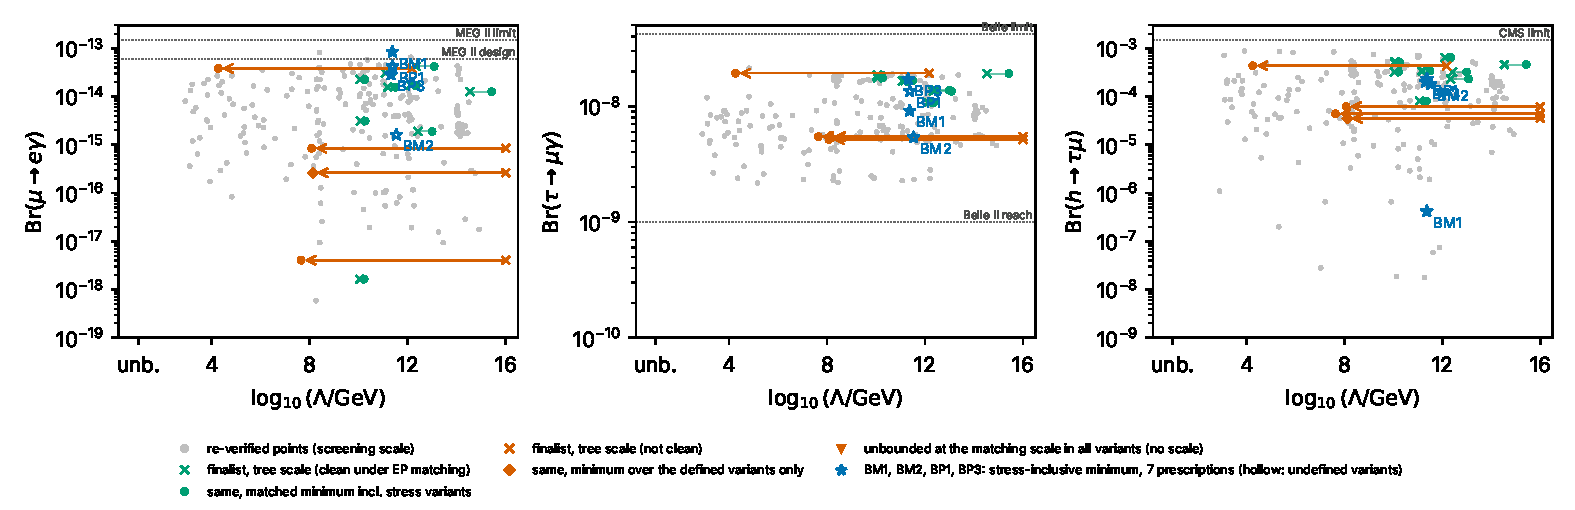
\includegraphics[width=\textwidth]{figures/fig_prod1_rates.pdf}
\caption{LFV rates versus scale. Grey: re-verified points with their screening scale (tree-level boundary, $13$ variants). Crosses: the $37$ finalists flagged robust by the proxy, at their tree-level scale; circles: their minimum over the re-matched variants including the stress variants (effective-potential matching; green clean, orange not clean); diamonds: minimum over the defined variants only when some variants have no scale; triangles at the left edge: finalists whose matched boundary is unbounded at the matching scale in all variants (no scale, a separate category and not a value); arrows: collapse of the tree scale under the matched stress (C39, C40). Stars: BM1, BM2, BP1 and BP3 at the stress-inclusive minimum over the defined variants of all seven prescriptions (hollow: some variants undefined). Dotted lines: present limits and projected sensitivities of Table~\ref{tab:inputs}.}\label{fig:prod1}\end{figure*}

\paragraph{Reference witnesses and benchmarks.} Table~\ref{tab:bm} lists four validated points whose columns are read from the same kind of record: BM1 and BM2, the two starting points of the exploration, and BP1 and BP3, finalists C42 and C35 of the production run (the latter two validated with all seven matching prescriptions of \ref{app:val}, all Yukawa couplings evolved at the tree boundary and with the $h$-pole matched boundaries, a vacuum search with $1527$ starts and the $H^\pm W^\mp\gamma$ envelope). We call a point \emph{robust} if all seven matching prescriptions are complete, i.e.\ every one of the $13$ variants of each prescription has a defined scale, and \emph{EP-clean only} if the effective-potential prescription is complete with a stress minimum of at least $10^{10}$~GeV but not all seven are. Robust means that every variant tested yields a scale; it does not mean that the scale is known to better than the uncertainties of Sec.~\ref{sec:disc}. BM1 is not among the ranked finalists because it is a starting point, not because it failed a test. BP1 is the clean finalist with the largest $\Br(\mu\to e\gamma)$ and BP3 has the highest matched stress minimum among the clean finalists with $\Br(\tau\to\mu\gamma)\ge1.7\times10^{-8}$; the selection is by hand and not unique. Two further validated finalists are in the repository and not discussed here: C43, which is redundant with BP1, and C57, which has $\Br(h\to\tau\mu)=6.6\times10^{-4}$ but a singlet-direction margin $\lambda_h=0.005$, a HiggsBounds ratio of $0.994$ for $H$ and an unbounded matched boundary in two prescriptions, so that we do not use it as a benchmark.

\textbf{BM1} has $\Br(\mu\to e\gamma)=8.5\times10^{-14}$, independent of the $H^\pm W^\mp\gamma$ set and above the MEG~II design sensitivity ($6\times10^{-14}$, not a discovery sensitivity), all seven prescriptions complete, a tree-level minimum scale of $10^{11.6}$~GeV and, over all prescriptions and including the stress variants, $10^{11.37}$~GeV (the prescription with the heavy evaluation of the $h$--$H$ element). Its conservative tree-level margin is $0.026$, its smallest matched boundedness margin $0.015$ and its $\chi^2$ margin $0.85$; these margins are small. The nominal $\Br(\tau\to\mu\gamma)=9.1\times10^{-9}$ of BM1 depends on the $H^\pm W^\mp\gamma$ set: it is $3.9\times10^{-9}$ without it and $9.1\times10^{-10}$ with its sign reversed (Fig.~\ref{fig:hw}; the rates are exactly quadratic in the multiplier $s$, and the minimum over $|s|\le1$ is $9.05\times10^{-10}$ for BM1 and $7.7\times10^{-10}$ for BM2, \texttt{gate2/hw\_envelope.py}). The record of BM1 was produced with the code of the first release, before the campaign code.

\textbf{BP3} is the robust campaign benchmark: all seven prescriptions are complete, the tree-level boundedness margin is $0.077$ and the largest quartic $0.82$. The minimum over the prescriptions, including the stress variants, with the production (top-only) renormalisation-group equations is $10^{11.31}$~GeV (the prescription with the heavy evaluation of the $h$--$H$ element), and the all-Yukawa runs combined with the three $h$-pole matched boundaries give $10^{11.35}$--$10^{11.36}$~GeV; the combined run for the other four prescriptions has not been done. It has $\Br(\tau\to\mu\gamma)=1.7\times10^{-8}$ (nominal; $2.3\times10^{-9}$ to $1.7\times10^{-8}$ over $|s|\le1$ of the $H^\pm W^\mp\gamma$ set), $\Br(\mu\to e\gamma)=2.9\times10^{-14}$ and $\Br(h\to\tau\mu)=2.0\times10^{-4}$. Its lighter charged scalar ($476$~GeV, $\Br(\mu\nu)=0.2\%$) lies inside the domain of the Drell--Yan recast and passes with a weight of $10^{-5}$ against a threshold of $1.2$, while its heavier scalar is outside the domain. Its smallest matched boundedness margin is $0.025$, its $\chi^2$ margin is $0.07$ and the HiggsBounds ratio of $H$ and $A$ is $0.93$, so BP3 is the thinnest of the benchmarks experimentally.

\textbf{BP1} has $\Br(\mu\to e\gamma)=4.2\times10^{-14}$, independent of the $H^\pm W^\mp\gamma$ set and below the MEG~II design sensitivity, $\Br(\tau\to\mu\gamma)=1.3\times10^{-8}$ ($1.8\times10^{-9}$ to $1.3\times10^{-8}$) and $\Br(h\to\tau\mu)=2.3\times10^{-4}$, the three together. It is the largest rate among the clean finalists and not a robust point: in the prescription with the heavy evaluation of the $h$--$H$ element one of the $13$ variants (heavy-scale boundary, $\times2$) is unbounded at the matching scale (margin $-0.003$), so BP1 has no robust scale. The six complete prescriptions give matched scales of $10^{13.5}$--$10^{14.3}$~GeV and stress minima of $10^{12.1}$--$10^{13.1}$~GeV, and the defined variants of the seventh $10^{12.3}$ and $10^{11.4}$~GeV; its $\chi^2$ margin is $0.52$. \textbf{BM2} has $\Br(h\to\tau\mu)=1.8\times10^{-4}$ (a factor $8$ below the CMS limit), $\Br(\tau\to\mu\gamma)=5.4\times10^{-9}$ and $\Br(\mu\to e\gamma)=1.6\times10^{-15}$ and is EP-clean only: its tree-level minimum scale is $10^{12.1}$~GeV, but in the symmetric and heavy evaluations of the $h$--$H$ element $12$ of the $13$ variants are unbounded at the matching scale (default-boundary margins $-0.026$ and $-0.037$; the smallest matched margin over all prescriptions and variants is $-0.12$), because the one-loop definition of the $h$--$H$ mixing shifts $c_{\beta-\alpha}=0.020$ by about $0.01$ (\ref{app:val}). BM2 is therefore a demonstration only under the on-shell-$h$ identification of the mixing, and its $\chi^2$ margin is $0.52$.

The $\chi^2$ of BM1, BM2, BP1 and BP3 ($13.03$, $13.35$, $13.36$, $13.81$) lie $0.85$, $0.52$, $0.52$ and $0.07$ below the limit of $13.88$: the chains end at the edge of the $\chi^2$-compatible region. The reference matters: the limit uses the minimum $10.04$ with the free quartics in $|\lambda|\le3$, reached at the edge of that box. Refitting with $|\lambda_{7,8,10}|\le1$ and $\le0.75$ (the range of the benchmarks) gives minima of $10.72$ and $10.86$ and margins of $1.5$ and $1.2$ ($1.7$ and $1.4$) for BM1 and BM2, and with the DESI-DR2 bound $\sum m_\nu<0.0642$~eV the refit minimum is $10.74$ and the margins of BM1 and BM2 stay at $0.8$ and $0.5$ (Table~\ref{tab:ref}). All four points under each input variation, each against the refit minimum of the same variation, are in Table~\ref{tab:inp}: the exact $z_{0.975}$, the DESI-DR2 bound and the removal of the cosmological term change the margins by at most $0.06$ (the margin of BP3 under DR2 is $0.007$), while the RPP~2026 oblique fit leaves BP1 and BP3 inside the limit, by $0.37$ and $0.80$, and puts BM1 and BM2 outside it, by $0.81$ and $7.5$; BM1 and BM2 were not refitted under it. The rates and collider quantities of these points are computed from the input spectrum and mixing; the matching and stress tests change only the boundary quartics of the evolution and test the scalar consistency of the point, not a one-loop corrected prediction of its observables.

% rows generated by gate2/make_table_prod1.py (columns BM1 BM2 BP1 BP3; rows tau->e gamma, mu->3e, d_e, sum m_nu and the individual variant rows omitted)
\begin{table*}[t]\centering\scriptsize\setlength{\tabcolsep}{2.5pt}
\begin{tabular}{p{5.0cm}cccc}\toprule
 & BM1 & BM2 & BP1 & BP3\\\midrule
$m_H,\ m_A$ [GeV] & 652, 629 & 868, 871 & 561, 549 & 489, 482\\
$m_{h_1^+},\ m_{h_2^+}$ [GeV] & 612, 869 & 573, 896 & 536, 846 & 476, 798\\
$\tan\beta$, $c_{\beta-\alpha}$ & 0.43, 0.0009 & 0.43, 0.0203 & 0.43, 0.0219 & 0.43, 0.0201\\
$\cos\varphi$, $\mu/v$ & 0.94, 2.92 & 0.34, 3.51 & 0.97, 2.50 & 0.97, 2.13\\
$\lambda_1,\lambda_2,\lambda_3$ & 0.26, 0.19, 0.73 & 0.26, 0.27, 0.38 & 0.26, 0.15, 0.73 & 0.26, 0.28, 0.82\\
$\lambda_4,\lambda_5,\lambda_6$ & -0.36, 0.48, -0.01 & 0.19, -0.08, -0.25 & -0.26, 0.23, -0.11 & -0.42, 0.11, -0.07\\
$\lambda_7,\lambda_8,\lambda_9$ & 0.05, -0.14, 0.25 & 0.25, 0.07, 0.32 & 0.10, -0.26, 0.13 & 0.10, -0.24, 0.37\\
$\lambda_{10}$, $\lambda_h$ & 0.11, 0.2741 & 0.09, 0.0200 & 0.04, 0.2954 & 0.03, 0.3166\\
$\max|Y_2|$, $|f_{\mu\tau}|$ & 0.026, $1.5\times10^{-6}$ & 0.025, $1.3\times10^{-6}$ & 0.026, $1.5\times10^{-6}$ & 0.026, $1.5\times10^{-6}$\\
\midrule
\midrule
$\Br(\mu\to e\gamma)$ & $8.5\times10^{-14}$ & $1.6\times10^{-15}$ & $4.2\times10^{-14}$ & $2.9\times10^{-14}$\\
$\Br(\tau\to\mu\gamma)$ & $9.1\times10^{-9}$ & $5.4\times10^{-9}$ & $1.3\times10^{-8}$ & $1.7\times10^{-8}$\\
\quad range for $|s|\le1$ & $9.1\times10^{-10}$--$9.1\times10^{-9}$ & $7.7\times10^{-10}$--$5.4\times10^{-9}$ & $1.8\times10^{-9}$--$1.3\times10^{-8}$ & $2.3\times10^{-9}$--$1.7\times10^{-8}$\\
$\Br(h\to\tau\mu)$ & $4.2\times10^{-7}$ & $1.8\times10^{-4}$ & $2.3\times10^{-4}$ & $2.0\times10^{-4}$\\
$B\to X_s\gamma$ [$10^{-4}$] & 3.27 & 3.30 & 3.26 & 3.24\\
$\chi^2$ ($\chi^2_{\min}=10.04$, limit $13.88$) & 13.03 & 13.35 & 13.36 & 13.81\\
$\Delta\chi^2_{\rm HS}=\chi^2_{\rm HS}-153.72$, HiggsBounds & -0.04, allowed & -0.76, allowed & -0.83, allowed & -0.77, allowed\\
Drell--Yan screen & PASS & PASS & PASS & PASS\\
\midrule
\midrule
$\log_{10}(\Lambda/\mathrm{GeV})$, default inputs & 12.75 & 13.51 & 13.94 & 12.33\\
minimum over the 13 prescribed variants & 11.6 & 12.1 & 12.3 & 11.2\\
\quad with all Yukawa couplings evolved (tree boundary) & 11.6 & 12.1 & 12.3 & 11.2\\
\quad one-loop (effective-potential) matching: re-matched variants & 12.5 & 13.3 & 14.3 & 12.2\\
\quad \qquad including the stress variants & 11.5 & 12.2 & 13.1 & 11.4\\
\quad momentum-dependent matching, $h$ pole (3 prescriptions): re-matched variants & 12.3--12.6 & 12.5--13.0 & 14.2--14.3 & 12.2\\
\quad \qquad including the stress variants & 11.4--11.6 & 11.5--12.0 & 12.9--13.0 & 11.4\\
\quad momentum-dependent matching, all 6 prescriptions: re-matched variants & 11.8--12.9 & 12.4--13.0$^{(24)}$ & 12.3--14.3$^{(1)}$ & 12.2--12.3\\
\quad \qquad including the stress variants & 11.4--12.0 & 11.5--12.5 & 11.4--13.0 & 11.3--11.4\\
\quad $h$-pole matching and all Yukawa couplings & 11.4--11.6 & 11.5--12.0 & 12.9--13.0 & 11.4\\
complete prescriptions (of 7), status & 7, robust & 5, EP-clean only & 6, EP-clean only & 7, robust\\
conservative tree margin $\min(V_{\rm red},\lambda_h)$, min. matched $V_{\rm red}$ margin & 0.026, 0.015 & 0.020, -0.123 & 0.058, -0.003 & 0.077, 0.025\\
first failure & unitarity & unitarity & unitarity & unitarity\\
no deeper minimum found (1527 starts) & EW & EW & EW & EW\\
\bottomrule\end{tabular}
\caption{Reference points (BM1, BM2; starts~0 and 1 of the campaign) and campaign benchmarks (BP1, BP3; finalists C42 and C35 of the production run). All limits hold as hard cuts and $\chi^2\le\chi^2_{\min}+3.84$ with the free quartics of the table (the statistic of Eq.~\eqref{eq:chi2}; a working criterion, not a calibrated confidence level); HiggsSignals ($\chi^2$ not worse than the Standard-Model-like value $153.72$ of the same 159 observables by more than $3.84$) and HiggsBounds (both charged scalars with $\ell\nu$, $tb$, $Wh$, $WH$, $WA$ and $h_1^+Z$ decays) are evaluated with the quartics of the table. $\Br(\tau\to\mu\gamma)$ is the nominal value; the next row gives its range over an overall multiplier $|s|\le1$ of the $H^\pm W^\mp\gamma$ amplitude. The cutoff $\Lambda$ is the scale at which the first of boundedness, perturbativity ($|\lambda_i|<4\pi$) or unitarity ($|\Lambda_{2\to2}|<8\pi$) fails, located by bisection on a grid of $100$ scales per decade; the matched rows start the evolution at $\mu_0\ge m_t$ with one-loop Standard-Model couplings run from $m_t$. The rows below the minimum over the $13$ variants repeat it with all Yukawa couplings evolved at the tree boundary (third-generation quarks and all lepton Yukawa couplings; the first two quark generations are neglected); with the one-loop effective-potential matching of the boundary quartics; with the matching with momentum-dependent self-energies in the three prescriptions that evaluate the $h$--$H$ mixing at the $h$ pole (\ref{app:val}) and in all six prescriptions (including the symmetric and heavy evaluations of the $h$--$H$ element), each as the minimum over the re-matched variants and, on the next row, including the stress variants (quartics $\times0.9$, $\times1.1$, arbitrary rescalings that are not re-matchings and not calculated threshold corrections); and the all-Yukawa runs combined with the three $h$-pole matched boundaries. None of these rows is part of the gate and all matching runs use the production (top-only) renormalisation-group equations. Ranges are over the prescriptions of the row and use only variants with a defined scale; a number in parentheses is the number of variants, summed over the prescriptions of the row, that have no scale because the matched boundary is unbounded or non-perturbative at the matching scale. The row ``complete prescriptions'' gives the number of the seven prescriptions in which all $13$ variants have a scale and the status (robust: all seven complete; EP-clean only: effective-potential prescription complete with stress minimum $\ge10^{10}$~GeV, not all seven complete); the margin row gives the conservative tree-level margin $\min(V_{\rm red},\lambda_h)$ and the smallest matched $V_{\rm red}$ margin over all prescriptions and variants. The robust scales (minimum over all seven prescriptions and the stress variants) are $10^{11.37}$~GeV for BM1 and $10^{11.31}$~GeV for BP3; BM2 and BP1 have none. The charged scalars of BM1, BM2 and BP1 lie above $500$~GeV, outside the domain of the Drell--Yan recast ($\ell\nu$ branching ratios below $0.3\%$): their PASS means not tested by the recast; BP3 has $m_{h_1^+}=476$~GeV, inside the domain, and passes it. Full records are in the repository.}\label{tab:bm}\end{table*}

\paragraph{Why these points survive.} The benchmarks share a pattern (Table~\ref{tab:bm}). All scalars lie at $0.48$--$0.9$~TeV with no large hierarchy, the second doublet is nearly degenerate ($m_H\simeq m_A$) and close to alignment ($|c_{\beta-\alpha}|\le0.022$). The lighter charged scalar ($476$--$612$~GeV) decays to $tb$ with a branching ratio of $0.994$--$0.998$, which evades the slepton-like Drell--Yan limits that exclude lighter states with $\mu\nu$ decays. All quartics are below $0.85$ in magnitude at the matching scale. The LFV rates are carried by $Y_2$ entries of a few times $10^{-2}$: in the component amplitudes of the benchmark records $\mu\to e\gamma$ comes from the one-loop neutral-scalar diagram with a $\tau$ in the loop and $\tau\to\mu\gamma$ from the Barr--Zee fermion loops, with the $H^\pm W^\mp\gamma$ and $W$ Barr--Zee loops large and the one-loop and charged-scalar loops negligible. The neutrino masses are set by $f\sim10^{-6}$ times $Y_2$ through Eq.~\eqref{eq:mnu}, which leaves $Y_2$ free to be sizeable. None of this requires large quartics. The Higgs LFV rate requires $c_{\beta-\alpha}\ne0$, $\Gamma(h\to\tau\mu)\propto c_{\beta-\alpha}^2(|D_{\tau\mu}|^2+|D_{\mu\tau}|^2)$, with $c_{\beta-\alpha}\simeq-\lambda_6v^2/(m_H^2-m_h^2)$, so BM2 needs a larger $|\lambda_6|=0.25$; its tree-level minimum scale ($10^{12.1}$~GeV) is nevertheless not lower than that of BM1 ($10^{11.6}$~GeV), and the matched runs show BM2 to be the more fragile point, but two points do not establish a trade-off between the Higgs LFV rate and the reach. Fig.~\ref{fig:traj} compares the flow of BM1 and BM2 with an illustrative point that fails near $10^5$~GeV: the latter starts with quartics of order $2$ and reaches the unitarity limit quickly, while the benchmarks start below $0.85$. A conventional scan with $\lambda_2=\sqrt{4\pi}$ and order-one quartics, as in \HG{}, places the Landau pole near the TeV scale and does not sample this region.

\begin{figure*}[t]\centering
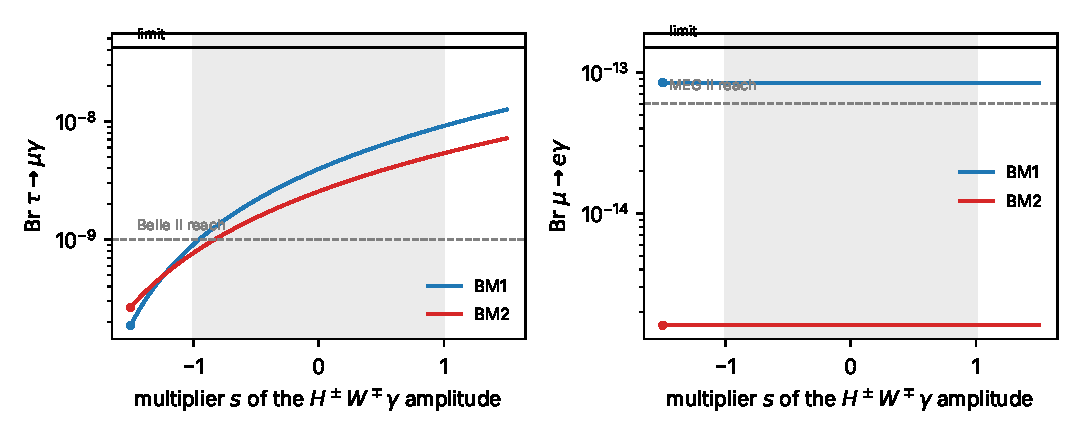
\includegraphics[width=0.49\textwidth]{fig_hw.pdf}\hfill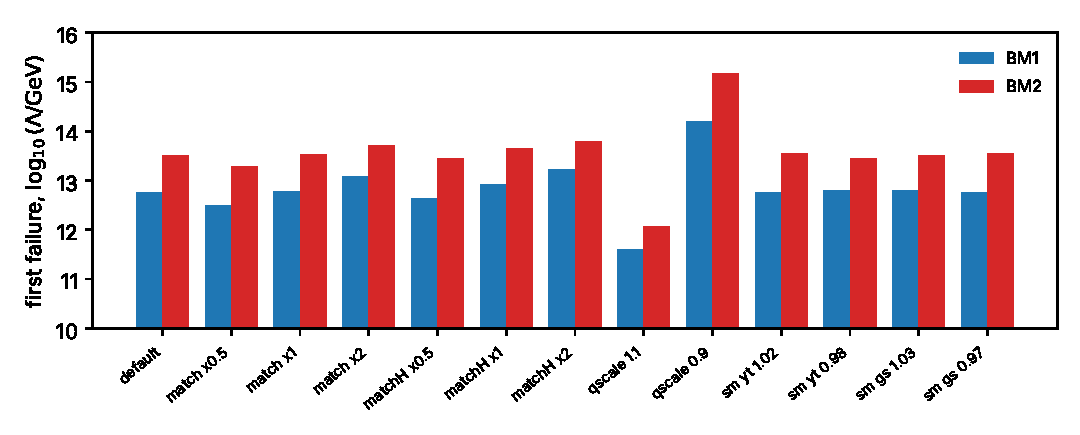
\includegraphics[width=0.49\textwidth]{fig_variants.pdf}
\caption{Left: $\Br(\tau\to\mu\gamma)$ and $\Br(\mu\to e\gamma)$ of BM1 and BM2 as functions of the multiplier $s$ of the $H^\pm W^\mp\gamma$ amplitude ($s=1$ is the nominal value; the shaded band is the range $|s|\le1$ used in the gate); the thin lines are the current limit and the projected reach. The $\tau\to\mu\gamma$ rate crosses the Belle~II reach near $s\simeq-1$; $\mu\to e\gamma$ is unaffected. Right: scale of the first failure for the 13 boundary variants (the minimum is the quoted scale).}\label{fig:hw}\label{fig:variants}
\end{figure*}

\begin{figure*}[t]\centering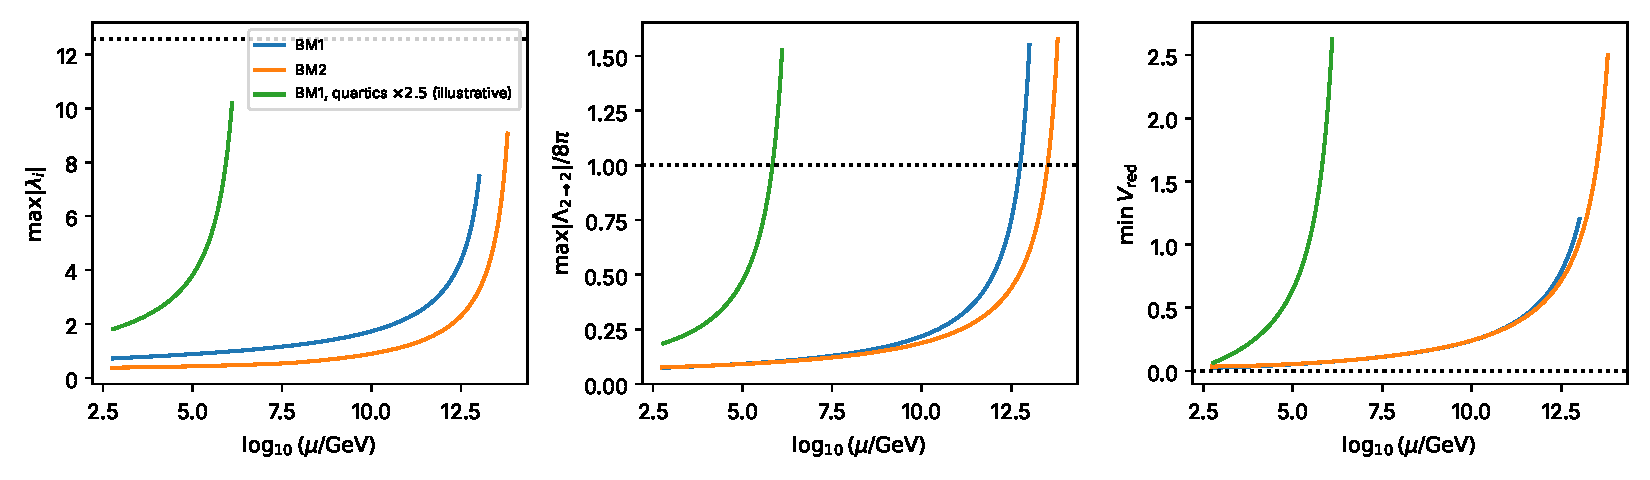
\includegraphics[width=0.9\textwidth]{figures/fig_trajectories.pdf}
\caption{One-loop flow for BM1, BM2 and, for contrast, BM1 with all quartics at the matching scale multiplied by $2.5$ (an illustrative point, not validated): largest quartic, largest $2\to2$ eigenvalue in units of $8\pi$, and minimum of $V_{\rm red}$ (Eq.~\eqref{eq:vred}).}\label{fig:traj}\end{figure*}

\section{Discussion and limitations}\label{sec:disc}
\begin{itemize}
\item \emph{Scope.} All results refer to the slice with the quark sector of \HG{}, $|\lambda_{3,4,5,6}|\le\sqrt{4\pi}$, $0.3\le\tan\beta$ (perturbative Yukawa couplings limit the physical domain to $\tan\beta<3.6$, Sec.~\ref{par:tanb}), $|f|,|Y_2|\le0.1$, and normal ordering. The slice is a restricted texture of the general model, and distant minima of the general texture are not explored; a local relaxation of the texture has not been repeated with the final treatment of the limits. The benchmarks prove existence within this setup; they do not bound the largest rate compatible with a given cutoff, and failing to find a point at a given cutoff is inconclusive. The boundedness penalties of the fit, taken from \HG{} (Sec.~\ref{sec:obs}), are not necessary conditions and restrict the scanned domain. The Yukawa perturbativity cut is entrywise on the couplings at the starting scale; along the flow the production gate tracks the running top couplings ($y_t$ and $\rho_t=r\,y_t$ must stay below $\sqrt{4\pi}$), while the bottom, tau and lepton Yukawa couplings and $f$ are evolved only in the separate complete-Yukawa run of \ref{app:val}. The texture zeros are regenerated by the running at the level of $2\times10^{-4}$ or below; their effect on the LFV rates of the near-limit points has not been evaluated.
\item \emph{Observables.} The conversion rate in the statistic and in the gate is the sum of (i) the neutral-scalar photon-penguin (monopole) term of Eqs.~(3.24)--(3.25) of \HG{}, (ii) the dipole-dominance estimate $\mathrm{CR}=\pi D^2(\Gamma_\mu/\Gamma_{\rm capt})\Br(\mu\to e\gamma)$ with the overlap integrals of Ref.~\cite{Kitano:2002mt} (ratios $2.7\times10^{-3}$ for Al and $3.9\times10^{-3}$ for Au) and (iii) the scalar-exchange terms, added as rates, i.e.\ without interference and without charged-scalar photon-penguin, $Z$-penguin or box terms. Since $\Br(\mu\to e\gamma)<1.5\times10^{-13}$ bounds the dipole part below $6\times10^{-16}$, far under the SINDRUM~II bound, no conversion rate is claimed; $\mu\to3e$ is a dipole-dominated estimate that enters no claim. Flavour observables beyond $b\to s\gamma$ (for example $B_s$ mixing, $B\to\tau\nu$ and $R_b$) were not evaluated; we expect them to be small for $\tan\beta<1$ and $M_{H^\pm}\gtrsim500$~GeV but have not checked. The Higgs signal strengths in the fit are an approximate Run-1 combination; current HiggsSignals data enter as a filter evaluated for each final point with its own quartics. The Drell--Yan constraint is a recast of slepton searches, not a dedicated analysis: for states above $500$~GeV it assigns zero cross section and returns PASS, which means that these states are not tested, not that they pass a meaningful test. BM1, BM2 and BP1 lie outside its domain (their leptonic branching ratios are below $2\times10^{-3}$, which makes slepton-like final states unlikely, but a pair rate has not been computed); BP3, with a charged scalar of $476$~GeV, is inside it and passes, its heavier scalar being outside. The $H^\pm\to tb$ search is covered by the HiggsBounds dataset (ATLAS, 139~fb$^{-1}$~\cite{ATLAS:2021upq}): the observed-to-limit ratios are $0.42$ for the $612$~GeV $h_1^+$ of BM1, $0.002$ for its $h_2^+$, and $0.05$ and $0.08$ for the two charged scalars of BM2; the decays of $H$, $A$ into three-body final states and $h_2^+\to h_1^+H/A$ are not included. The gate also requires all Yukawa-type couplings to be perturbative, $\max(|D_{ij}|,2|f_{ij}|,\sqrt2\tan\beta\,m_t/v)<\sqrt{4\pi}$; the benchmarks have $0.43$.
\item \emph{Tau rates.} The nominal $\tau\to\mu\gamma$ rates contain the $H^\pm W^\mp\gamma$ set of Ref.~\cite{Ilisie:2015tra} mapped onto the off-diagonal Zee couplings, and the $t$--$b$ subset dominates. The set is validated against GM2Calc in the diagonal $\Delta a_\mu$ of the aligned two-doublet model at the $10\%$ level (\ref{app:val}); the off-diagonal entries, the mixing of the charged scalars with the singlet and the two-loop flavour-violating amplitudes are not independently verified, and an independent one-loop calculation validates only the one-loop flavour-violating terms. The $\tau\to\mu\gamma$ rates are therefore model-dependent estimates, to be read with the variation of Fig.~\ref{fig:hw} (a factor of about $7$ between the nominal value and the minimum over $|s|\le1$ at BP3). $\Br(\mu\to e\gamma)$ and $\Br(h\to\tau\mu)$ do not depend on this set.
\item \emph{Sensitivity of $\mu\to e\gamma$ and $h\to\tau\mu$ to the spectrum.} Near alignment the off-diagonal couplings in Eq.~\eqref{eq:dipole} are $\Lambda^H\simeq-D/\sqrt2$ and $\Lambda^A=iD/\sqrt2$, so the internal-flip terms proportional to $\Lambda^{\varphi*}_{kj}\Lambda^{\varphi*}_{ik}$ and $\Lambda^\varphi_{jk}\Lambda^\varphi_{ki}$ have opposite signs for $H$ and $A$ and cancel at leading order for $m_H=m_A$; what remains is controlled by the difference of the loop functions of $H$ and $A$, i.e.\ by the splitting $m_H^2-m_A^2\simeq\lambda_5v^2$, and by the external-flip terms, which add. The benchmarks have splittings of $3$--$23$~GeV, of the order of one-loop corrections to the mass difference. We have not decomposed the amplitudes numerically, but we expect the $\mu\to e\gamma$ values of the benchmarks to be sensitive to the radiative corrections to the $H$--$A$ splitting; they are values for the tree-level spectrum. For $h\to\tau\mu$ the one-loop definition of the $h$--$H$ mixing moves $c_{\beta-\alpha}$ by about $0.01$ at BM2, comparable to $c_{\beta-\alpha}=0.020$, and the rate is proportional to $c_{\beta-\alpha}^2$: for a shift of $\pm0.01$ it would change by a factor between about $0.25$ and $2.3$ (an estimate from the quoted shift). The evaluation of the $h$--$H$ element at the $h$ pole is one convention and not a unique physical definition of the on-shell mixing.
\item \emph{Renormalisation group and matching.} The scale is the first crossing of perturbativity, unitarity ($8\pi$) or boundedness in a one-loop flow whose boundary quartics are either the tree-level ones or the output of the one-loop matching of \ref{app:val}. The production flow omits the bottom, tau and lepton Yukawa couplings; evolving them together with $Y_2$ and $f$ changes the scales of BM1 and BM2 by less than $0.003$ decades. The matching is a one-loop, Landau-gauge, real-part calculation at the input point with fixed spectator quartics and a gauge-dependent effective-potential $v$, without widths, bottom and tau loops or two-loop terms; it is not an observable-based renormalisation scheme. The mixing prescriptions are conventions for the one-loop definition of the mixings and not independent physical theories, so a boundedness failure under one of them is a warning of sensitivity and not a physical exclusion of the pole spectrum, and the $\times0.9$ and $\times1.1$ rescalings are arbitrary stresses; neither is a calibrated uncertainty. The boundedness margins of the benchmarks ($0.015$--$0.08$) are of the order of the threshold shifts of the matching ($|\Delta\lambda_i|\le0.056$ in the effective-potential estimate, up to $0.1$ for $\lambda_{4,6}$ with the momentum dependence) and a single-quartic shift of about $0.1$ removes the boundedness of BM2; a physically consistent shift of $M_{H^\pm}$ by $-1\%$ at fixed $m_H$, $m_A$, $m_h$ and singlet mass, with $\lambda_4$ re-solved, lowers the scale of BM1 to $10^{11.1}$~GeV and $+0.5\%$ violates boundedness already at its boundary (\ref{app:val}). The scales quoted are therefore consistent with these corrections only in the sense that every tested variant yields a scale, and not as accurate predictions. A PyR@TE~3 two-loop check of the $\beta$ functions alone (\ref{app:val}) raises the first-failure scale of the reference points by $0.46$--$0.74$ in $\log_{10}$; it uses the tree-level boundary, top-only Yukawa effects and tree-level unitarity, has not been run for BP1 and BP3 or with matched boundaries, and we do not claim two-loop accuracy. Differences of a few tenths of a decade between scales in this paper are below this uncertainty. We make no claim for a UV completion.
\item \emph{Vacuum.} The vacuum test is a multistart search of the tree-level potential at the input spectrum that can miss distant minima: we state that no deeper minimum was found, not that the electroweak vacuum is the global minimum, and metastability is not considered. The test is not a check of the matched effective potential, and a matched tree-level potential is not automatically stationary at the input field value because the matching uses loop tadpoles; a coherent one-loop vacuum analysis is not done. The boundedness test is an exact reduction over the singlet direction and the angular variables followed by a numerical minimisation, not a certified one.
\item \emph{Experimental margins and inputs.} The $\chi^2$ margins to the limit are $0.85$ (BM1), $0.52$ (BM2), $0.52$ (BP1) and $0.07$ (BP3), and the largest HiggsBounds observed-to-limit ratios are $0.38$ (BM1), $0.15$ (BM2), $0.56$ (BP1) and $0.93$ for $H$ and $A$ (BP3). The requirement $\Delta\chi^2\le3.84$ above an approximate minimum at the edge of the box is a working criterion, not a calibrated confidence level, and the statistic is a surrogate (Sec.~\ref{sec:fit}). The fit uses the DESI~2024 bound $\sum m_\nu<0.072$~eV; the benchmarks ($0.0633$--$0.0635$~eV) lie below the DR2 combination ($0.0642$~eV) by a small margin. All four points were re-evaluated, each against the refit minimum of the same variation, with the exact factor $z_{0.975}$, the DESI-DR2 bound, the RPP~2026 oblique parameters, all three together, and without the cosmological term (Table~\ref{tab:inp}). The first, second and last change the margins by at most $0.06$, leaving BP3 inside the limit under DR2 by only $0.007$. With the RPP~2026 oblique fit BP1 and BP3 keep margins of $0.37$ and $0.80$, whereas BM1 and BM2 fall outside the limit ($-0.81$ and $-7.5$) and would have to be refitted, which we have not done. The HiggsTools datasets used (\texttt{hbdataset} master, \texttt{hsdataset} v1.1) are the released heads. The unreleased development branch of \texttt{hbdataset} (March 2026) adds the ATLAS $138$~fb$^{-1}$ $h\to\mu\tau$ limit~\cite{ATLAS:2023mvd}, stored there as $1.8\times10^{-4}$ although the abstract of that paper gives $0.18\%$; as stored it marks BP1 and BP3 excluded (observed-to-limit ratios $1.27$ and $1.10$), with $1.8\times10^{-3}$ the ratios are $0.13$ and $0.11$ and all four points are allowed. Theoretical robustness under the matching and stress tests and experimental robustness are different properties: BP3 is the robust point of the first kind and the thinnest of the second.
\item \emph{Campaign and statistics.} The exploration starts from five points, three of which were found by a search that rejected $117$ of $120$ random deformations, and the chains are not converged (no basin has $\hat R<1.1$ for all monitored quantities; the largest split $\hat R$ is $2.8$); it cannot say how large the region around the starting points is or whether other regions exist, and chains at $L=14$ were sparse after the pilots showed that the starts cannot climb there, so a failure to find larger scales is inconclusive. Start~0 duplicates the $L=-1$ and $L=0$ chains. Only the effective-potential matching was run for the $37$ flagged finalists, the $22$ other finalists and the remaining verified points were not screened, BM1 was not part of the ranking, and only four finalists received the full validation, so the maxima of the screened rates are not bounds and BP1 is the largest $\Br(\mu\to e\gamma)$ among the clean finalists, not the largest robust rate (BM1 has the larger robust rate). The limits are represented by an approximate continuous likelihood, the ordering $\Delta\chi^2$ is a fit statistic, and nested sampling did not converge on the multimodal posterior, so no credible intervals are given.
\end{itemize}

\section{Conclusions}
On the restricted lepton-Yukawa slice of the Zee model, extended by a free $\lambda_4$, requiring the scalar sector to remain bounded from below, perturbative and unitary under one-loop running, with no deeper tree-level minimum found than the electroweak vacuum, removes points with quartic couplings of order one at the electroweak scale. It does not remove observable lepton flavour violation. A Metropolis exploration of $2089$ chains around five starting points finds re-verified points that pass a fail-closed gate and have tree-level scales up to $10^{14.5}$~GeV with $\Br(\tau\to\mu\gamma)\gtrsim10^{-8}$, with $\Br(h\to\tau\mu)\gtrsim10^{-4}$ or with $\Br(\mu\to e\gamma)\gtrsim3\times10^{-14}$. The tree-level scale overstates the reach, however: of the $37$ finalists flagged by a matched-margin proxy only $21$ survive an effective-potential matching in all variants, and the six points with $\Br(\mu\to e\gamma)\simeq1.2\times10^{-13}$, just below the MEG~II limit, are either unbounded at the matching scale (four) or fail below $10^{6.4}$~GeV under a $10\%$ rescaling of the quartics (two). Two witnesses retain every variant of all seven tested matching prescriptions: the reference point BM1, with $\Br(\mu\to e\gamma)=8.5\times10^{-14}$, above the MEG~II design sensitivity, and the benchmark BP3, with $\Br(\tau\to\mu\gamma)=1.7\times10^{-8}$ (nominal; $2.3\times10^{-9}$ to $1.7\times10^{-8}$ over the range of the $H^\pm W^\mp\gamma$ amplitude), $\Br(\mu\to e\gamma)=2.9\times10^{-14}$ and $\Br(h\to\tau\mu)=2.0\times10^{-4}$, at scales of $10^{11.4}$ and $10^{11.3}$~GeV (minimum over the prescriptions and stress variants). BP1, with the largest $\Br(\mu\to e\gamma)=4.2\times10^{-14}$ among the clean finalists, has one undefined variant in one prescription, and BM2, with $\Br(h\to\tau\mu)=1.8\times10^{-4}$, depends on the on-shell-$h$ identification of the mixing. These are one-loop, approximate-matching existence demonstrations, not bounds and not predictions of corrected observables: the boundedness and $\chi^2$ margins are small, the $\tau\to\mu\gamma$ rates rest on a transcribed amplitude, and the $\mu\to e\gamma$ rates are tree-spectrum values near a cancellation between $H$ and $A$. The points rely on a heavy, nearly degenerate and aligned second doublet, a charged scalar at $0.5$--$0.6$~TeV decaying to $tb$ and small quartic couplings, with the LFV carried by the doublet Yukawa couplings and the neutrino masses by a small singlet coupling. An LFV signal in this model therefore does not by itself point to a low cutoff. Whether comparable rates survive to the GUT scale remains open: no candidate with matched validation reaches it. The chains are not converged, the benchmarks lie at the edge of the $\chi^2$-compatible region (BM1 and BM2 lie outside it with the RPP~2026 oblique fit, and BP3 is inside it by $0.007$ with the DESI-DR2 bound). The code, the campaign records and the validation against PyR@TE are available at \url{https://github.com/aalida0/Zee-RG}.

\begin{acknowledgements}The work of A.~Alida is funded by the National Center for Scientific and Technical Research (CNRST) under the PhD-Associate Scholarship (PASS).\end{acknowledgements}

\appendix
\section{One-loop $\beta$ functions of the quartics}\label{app:rge}
With $t=\ln\mu$, $16\pi^2\,d\lambda_i/dt=\beta_i$, real couplings, the potential of Eq.~(1), $g_1$ the hypercharge coupling (no GUT normalisation) and the top quark coupled to $H_1$ with $y_t$ and to $H_2$ with $\rho_t$ in the Higgs basis,
\begin{align}
\beta_{1}&=12\lambda_1^2 +4\lambda_3^2 +4\lambda_3\lambda_4\nonumber\\
&\quad +2\lambda_4^2 +2\lambda_5^2 +24\lambda_6^2\nonumber\\
&\quad +2\lambda_8^2 +12y_t^2\lambda_1 +12y_t\rho_t\lambda_6\nonumber\\
&\quad -3g_1^2\lambda_1 -9g_2^2\lambda_1 -12y_t^4\nonumber\\
&\quad +\tfrac{3}{4}g_1^4 +\tfrac{3}{2}g_1^2g_2^2 +\tfrac{9}{4}g_2^4\\
\beta_{2}&=12\lambda_2^2 +4\lambda_3^2 +4\lambda_3\lambda_4\nonumber\\
&\quad +2\lambda_4^2 +2\lambda_5^2 +24\lambda_7^2\nonumber\\
&\quad +2\lambda_9^2 +12y_t\rho_t\lambda_7 +12\rho_t^2\lambda_2\nonumber\\
&\quad -3g_1^2\lambda_2 -9g_2^2\lambda_2 -12\rho_t^4\nonumber\\
&\quad +\tfrac{3}{4}g_1^4 +\tfrac{3}{2}g_1^2g_2^2 +\tfrac{9}{4}g_2^4\\
\beta_{3}&=6\lambda_1\lambda_3 +2\lambda_1\lambda_4 +6\lambda_2\lambda_3\nonumber\\
&\quad +2\lambda_2\lambda_4 +4\lambda_3^2 +2\lambda_4^2\nonumber\\
&\quad +2\lambda_5^2 +4\lambda_6^2 +16\lambda_6\lambda_7\nonumber\\
&\quad +4\lambda_7^2 +2\lambda_8\lambda_9 +6y_t^2\lambda_3\nonumber\\
&\quad +6y_t\rho_t\lambda_6 +6y_t\rho_t\lambda_7 +6\rho_t^2\lambda_3\nonumber\\
&\quad -3g_1^2\lambda_3 -9g_2^2\lambda_3 -12y_t^2\rho_t^2\nonumber\\
&\quad +\tfrac{3}{4}g_1^4 -\tfrac{3}{2}g_1^2g_2^2 +\tfrac{9}{4}g_2^4\\
\beta_{4}&=2\lambda_1\lambda_4 +2\lambda_2\lambda_4 +8\lambda_3\lambda_4\nonumber\\
&\quad +4\lambda_4^2 +8\lambda_5^2 +10\lambda_6^2\nonumber\\
&\quad +4\lambda_6\lambda_7 +10\lambda_7^2 +2\lambda_{10}^2\nonumber\\
&\quad +6y_t^2\lambda_4 +6y_t\rho_t\lambda_6 +6y_t\rho_t\lambda_7\nonumber\\
&\quad +6\rho_t^2\lambda_4 -3g_1^2\lambda_4 -9g_2^2\lambda_4\nonumber\\
&\quad -12y_t^2\rho_t^2 +3g_1^2g_2^2\\
\beta_{5}&=2\lambda_1\lambda_5 +2\lambda_2\lambda_5 +8\lambda_3\lambda_5\nonumber\\
&\quad +12\lambda_4\lambda_5 +10\lambda_6^2 +4\lambda_6\lambda_7\nonumber\\
&\quad +10\lambda_7^2 +2\lambda_{10}^2 +6y_t^2\lambda_5\nonumber\\
&\quad +6y_t\rho_t\lambda_6 +6y_t\rho_t\lambda_7 +6\rho_t^2\lambda_5\nonumber\\
&\quad -3g_1^2\lambda_5 -9g_2^2\lambda_5 -12y_t^2\rho_t^2\\
\beta_{6}&=12\lambda_1\lambda_6 +6\lambda_3\lambda_6 +6\lambda_3\lambda_7\nonumber\\
&\quad +8\lambda_4\lambda_6 +4\lambda_4\lambda_7 +10\lambda_5\lambda_6\nonumber\\
&\quad +2\lambda_5\lambda_7 +2\lambda_8\lambda_{10} +9y_t^2\lambda_6\nonumber\\
&\quad +3y_t\rho_t\lambda_1 +3y_t\rho_t\lambda_3 +3y_t\rho_t\lambda_4\nonumber\\
&\quad +3y_t\rho_t\lambda_5 +3\rho_t^2\lambda_6 -3g_1^2\lambda_6\nonumber\\
&\quad -9g_2^2\lambda_6 -12y_t^3\rho_t\\
\beta_{7}&=12\lambda_2\lambda_7 +6\lambda_3\lambda_6 +6\lambda_3\lambda_7\nonumber\\
&\quad +4\lambda_4\lambda_6 +8\lambda_4\lambda_7 +2\lambda_5\lambda_6\nonumber\\
&\quad +10\lambda_5\lambda_7 +2\lambda_9\lambda_{10} +3y_t^2\lambda_7\nonumber\\
&\quad +3y_t\rho_t\lambda_2 +3y_t\rho_t\lambda_3 +3y_t\rho_t\lambda_4\nonumber\\
&\quad +3y_t\rho_t\lambda_5 +9\rho_t^2\lambda_7 -3g_1^2\lambda_7\nonumber\\
&\quad -9g_2^2\lambda_7 -12y_t\rho_t^3\\
\beta_{8}&=6\lambda_1\lambda_8 +4\lambda_3\lambda_9 +2\lambda_4\lambda_9\nonumber\\
&\quad +12\lambda_6\lambda_{10} +4\lambda_8^2 +8\lambda_8\lambda_h\nonumber\\
&\quad +4\lambda_{10}^2 +6y_t^2\lambda_8 +6y_t\rho_t\lambda_{10}\nonumber\\
&\quad -\tfrac{15}{2}g_1^2\lambda_8 -\tfrac{9}{2}g_2^2\lambda_8 +3g_1^4\\
\beta_{9}&=6\lambda_2\lambda_9 +4\lambda_3\lambda_8 +2\lambda_4\lambda_8\nonumber\\
&\quad +12\lambda_7\lambda_{10} +4\lambda_9^2 +8\lambda_9\lambda_h\nonumber\\
&\quad +4\lambda_{10}^2 +6y_t\rho_t\lambda_{10} +6\rho_t^2\lambda_9\nonumber\\
&\quad -\tfrac{15}{2}g_1^2\lambda_9 -\tfrac{9}{2}g_2^2\lambda_9 +3g_1^4\\
\beta_{10}&=2\lambda_3\lambda_{10} +4\lambda_4\lambda_{10} +6\lambda_5\lambda_{10}\nonumber\\
&\quad +6\lambda_6\lambda_8 +6\lambda_7\lambda_9 +4\lambda_8\lambda_{10}\nonumber\\
&\quad +4\lambda_9\lambda_{10} +8\lambda_{10}\lambda_h +3y_t^2\lambda_{10}\nonumber\\
&\quad +3y_t\rho_t\lambda_8 +3y_t\rho_t\lambda_9 +3\rho_t^2\lambda_{10}\nonumber\\
&\quad -\tfrac{15}{2}g_1^2\lambda_{10} -\tfrac{9}{2}g_2^2\lambda_{10}\\
\beta_{h}&=2\lambda_8^2 +2\lambda_9^2 +4\lambda_{10}^2\nonumber\\
&\quad +20\lambda_h^2 -12g_1^2\lambda_h +6g_1^4
\end{align}
These expressions were generated with PyR@TE~3~\cite{Sartore:2020gou} from the model file in the repository and agree with our implementation to $6\times10^{-13}$ (Sec.~\ref{sec:rg}). In addition $16\pi^2\,dy_t/dt=y_t[\tfrac92(y_t^2+\rho_t^2)-8g_3^2-\tfrac94g_2^2-\tfrac{17}{12}g_1^2]$ and the same equation holds for $\rho_t$ with $y_t\leftrightarrow\rho_t$, so that $\rho_t/y_t$ is constant at one loop.

\section{Validation and robustness summary}\label{app:val}
This appendix collects, in one place, the checks behind the statements of the main text, with what was and was not done. Files refer to the repository.

\paragraph{Independent check of the $H^\pm W^\mp\gamma$ set.} We compare the diagonal $\Delta a_\mu$ of our complete dipole code (all one-loop terms and all Barr--Zee sets, SM Higgs subtracted) with GM2Calc~2~\cite{Athron:2021evk}, which includes the full two-loop contribution of the aligned two-Higgs-doublet model, for exact alignment, $\tan\beta=1$, $\lambda_{6,7}=0$, $M^2=M_{H^\pm}^2$, $\varsigma_u=\varsigma_d=-1$ and $\varsigma_\ell=30$ (GM2Calc Yukawa type 5; the Yukawa conventions are the aligned ones of $\varsigma_u$, $\varsigma_d$, $\varsigma_\ell$ with the pseudoscalar couplings $-\varsigma_u$, $+\varsigma_{d,\ell}$ used in the code). Table~\ref{tab:gm2} shows that the code with the nominal set reproduces GM2Calc to $2$--$10\%$, while reversing the sign or removing the set is excluded; the $\varsigma_u$, $\varsigma_\ell$ dependence (the contribution is $\propto\varsigma_u\varsigma_\ell$, checked for $(\varsigma_u,\varsigma_\ell)=(-1,30),(-1,-30),(-2,20),(-0.5,60)$) agree at the same level over $32$ configurations (\texttt{results/gm2calc\_check.json}). GM2Calc's own scheme choice (running couplings in the 2HDM) moves its result by $+7\%$ at $M_{H^\pm}=200$~GeV, which is the size of the residual. The check fixes sign, normalisation and mass dependence of the $t$--$b$ set (the other two sets vanish at exact alignment); a separate run for heavy charged scalars ($M_{H^\pm}=600$--$1000$~GeV, the benchmark range, \texttt{results/gm2calc\_check\_heavy.json}) gives code-to-GM2Calc ratios of $1.01$--$1.05$ for $s=+1$, $0.65$--$0.67$ for $s=0$ and $0.30$ for $s=-1$, so the sign and size are confirmed in the diagonal aligned limit at the relevant masses; it does not test the off-diagonal entries, which follow from the flavour structure (the operator is $\bar\ell_{L,J}\sigma F D_{JI}\ell_{R,I}$ with a flavour-universal coefficient). Away from alignment (\texttt{results/gm2calc\_check\_offalign.json}, $48$ configurations with $M_{H^\pm}=300$, $600$, $800$~GeV, $\tan\beta=0.5$--$2$, $\lambda_{6,7}\ne0$, both signs of $\varsigma_\ell$) the quartics $\lambda_{1\ldots5}$ of the $Z_2$-basis two-doublet potential are solved from the spectrum (reproducing GM2Calc's own values to $10^{-8}$), rotated to the Higgs basis, and the code, with its sets (5) and (6) and the trilinear couplings $s_{\beta-\alpha}\lambda_3+c_{\beta-\alpha}\lambda_7$, is compared with GM2Calc: the ratio is $0.99$--$1.07$ at $c_{\beta-\alpha}=0.014$ (the benchmarks have $|c_{\beta-\alpha}|\le0.021$), $1.00$--$1.08$ at $0.045$, $0.88$--$1.09$ at $0.14$ and $0.66$--$1.02$ at $0.31$, against $0.43$--$0.82$ and $0.14$--$0.56$ for the set removed or with reversed sign. The agreement therefore holds at the benchmark mixings, and degrades with $|c_{\beta-\alpha}|$ in a way we have not traced (GM2Calc contains pieces that the code does not); only the diagonal $\Delta a_\mu$ is compared. The gate still requires all limits for $0,\pm1$ times the whole set. \emph{Off-diagonal entries.} GM2Calc returns only the flavour-diagonal $\Delta a_\mu$, which probes the flavour-changing lepton couplings through the chirally enhanced $\tau$ (and $e$) loops, $\propto m_\mu m_\tau\,{\rm Re}(\rho_{\mu\tau}\rho_{\tau\mu})$. We feed the aligned type with a real flavour matrix $\Delta_\ell$ ($\rho_\ell=\sqrt2m_\ell\varsigma_\ell/v+\Delta_\ell$) to GM2Calc and the same matrix, as the matrix of couplings, to the amplitude matrices of the code (\texttt{results/gm2calc\_check\_offdiag.json}; $32$ configurations with $M_{H^\pm}=300$ and $600$~GeV, aligned and $s_{\beta-\alpha}=0.99$ with $\tan\beta=1,2$ and $\lambda_{6,7}\ne0$, $\varsigma_\ell=0,20,30$, and the patterns $(\mu\tau)$ with $\rho_{\mu\tau}\ne\rho_{\tau\mu}$ up to $0.3$ and $0.4$, $(e\mu)$ and a full matrix). The difference of $\Delta a_\mu$ with and without the off-diagonal entries agrees with GM2Calc to $0.999$--$1.002$ for the patterns with $\mu\tau$ entries and to $0.991$--$1.010$ in all cases (the largest deviations are for the tiny $e\mu$ terms); the total ratio is $0.99$--$1.07$ as in the diagonal check, and transposing the matrix changes the total by up to $3\%$, which fixes the index convention. This tests the chirality and flavour structure of the diagonal moment of the amplitude matrices, including the flavour sums; it does not test the flavour-violating moments ($\mu\to e\gamma$, $\tau\to\mu\gamma$), for which GM2Calc has no output, nor complex phases (its input blocks are real).
\begin{table*}[t]
\centering
\caption{$\Delta a_\mu$ ($10^{-9}$) of GM2Calc~2 and of our code with the $H^\pm W^\mp\gamma$ set multiplied by $s=+1$ (nominal), $0$ and $-1$ for the configuration of the text ($m_H$, $m_A$ in GeV).}\label{tab:gm2}
\begin{tabular}{lrrrrr}
\hline
$(M_{H^\pm},m_H,m_A)$ & GM2Calc & $s=+1$ & ratio & $s=0$ & $s=-1$\\
\hline
$(90,150,170)$ & $1.576$ & $1.430$ & $0.91$ & $0.917$ & $0.404$\\
$(200,250,250)$ & $1.106$ & $1.043$ & $0.94$ & $0.680$ & $0.317$\\
$(300,300,300)$ & $0.910$ & $0.873$ & $0.96$ & $0.590$ & $0.307$\\
$(400,420,430)$ & $0.680$ & $0.667$ & $0.98$ & $0.438$ & $0.209$\\
\hline
\end{tabular}
\end{table*}

\paragraph{Reference of the acceptance statements.} The acceptance limit is $\chi^2_{\min}+3.84$ with the minimum of the fit over the stated domain; the refit minima of the table were computed before the final update of the universality likelihood, which shifts them by at most $0.1$. Table~\ref{tab:ref} lists the refit minima for the variants of the free quartics ($\lambda_{7,8,10}$) and of the cosmological bound, each from a multi-start fit (63 starts, normal ordering) with the production statistic, and the resulting margins of the benchmarks ($\chi^2=13.03$ for BM1, $13.34$ for BM2; with the DESI-DR2 bound $13.79$ and $14.10$). The benchmarks are inside the acceptance region for every reference.
\begin{table*}[t]
\centering
\caption{Refit minima and benchmark margins $\chi^2_{\min}+3.84-\chi^2$.}\label{tab:ref}
\begin{tabular}{lccc}
\hline
Reference & $\chi^2_{\min}$ & BM1 & BM2\\
\hline
$|\lambda_{7,8,10}|\le3$ (fit, box edge) & $10.04$ & $0.79$ & $0.48$\\
$|\lambda_{7,8,10}|\le1$ & $10.72$ & $1.53$ & $1.23$\\
$|\lambda_{7,8,10}|\le0.75$ & $10.86$ & $1.67$ & $1.36$\\
DESI-DR2, $\sum m_\nu<0.0642$~eV, $|\lambda|\le3$ & $10.74$ & $0.79$ & $0.48$\\
\hline
\end{tabular}
\end{table*}

\paragraph{Input variations.} Table~\ref{tab:inp} lists the four points under each variation (\texttt{gate2/input\_sensitivity.py}); the reference minimum of each variation is a local refit (\texttt{gate2/refit\_hw.py}) from the $21$ stored minima of the multi-start fit, without random restarts, except for the first row, which is the $63$-start fit. Each variation changes the likelihood only through the quoted input, with $z_{0.975}=1.95996$ in place of $1.949$ for the half-normal limits, $\sum m_\nu<0.0642$~eV, the RPP~2026 free-$U$ values $S=0.018\pm0.095$, $T=0.04\pm0.12$, $U=-0.013\pm0.086$ with correlations $(0.91,-0.66,-0.88)$, and the cosmological term removed (limit $10^3$~eV). The oblique $\chi^2$ of the four points is $0.41$, $1.71$, $0.45$, $0.59$ with the fit values of the main text and $3.86$, $11.57$, $2.40$, $1.65$ with RPP~2026; their $T$ is $0.05$--$0.09$ and $S,U\simeq0$, so a positive $T$ with $S\simeq0$ is penalised by the strong $S$--$T$ correlation of the newer fit.
\begin{table*}[t]
\centering
\caption{Margins $\chi^2_{\min}+3.84-\chi^2$ of the four points under input variations; negative values lie outside the limit. The last row combines the exact $z_{0.975}$, DESI-DR2 and RPP~2026.}\label{tab:inp}
\begin{tabular}{lccccc}
\hline
Variation & $\chi^2_{\min}$ & BM1 & BM2 & BP1 & BP3\\
\hline
Fit of the main text & $10.04$ & $0.85$ & $0.52$ & $0.52$ & $0.07$\\
Exact $z_{0.975}$ & $10.07$ & $0.85$ & $0.53$ & $0.52$ & $0.07$\\
DESI-DR2, $\sum m_\nu<0.0642$~eV & $10.74$ & $0.79$ & $0.47$ & $0.46$ & $0.007$\\
RPP~2026 oblique parameters & $11.83$ & $-0.81$ & $-7.54$ & $0.37$ & $0.80$\\
Without cosmological term & $7.08$ & $0.84$ & $0.52$ & $0.50$ & $0.07$\\
All three updates & $12.64$ & $-0.80$ & $-7.54$ & $0.37$ & $0.80$\\
\hline
\end{tabular}
\end{table*}

\paragraph{Exact boundedness reduction.} For real quartics the angular variables can be removed exactly: at fixed $a$ the dependence on the imaginary part of $z$ is $(\lambda_4-\lambda_5)\,{\rm Im}(z)^2$, so the minimum lies at ${\rm Im}\,z=0$ or on the boundary of the disk, and the rest is a piecewise quadratic in ${\rm Re}\,z$ with the breakpoint $B=0$, whose minimum is found analytically; only the one-dimensional minimisation over $a$ is numerical. The reduction of Sec.~\ref{sec:rg} (\texttt{zee/bfb1d.py}, tests in \texttt{tests/test\_bfb1d.py}) reproduces the margins of both benchmarks and the grid verdict on $300$ random quartic sets, including the corner $\lambda_h=0$ (there the conditions $V_2\ge0$, $\lambda_8,\lambda_9\ge0$, $\lambda_8\lambda_9\ge\lambda_{10}^2$ are imposed).

\paragraph{Spectrum-consistent boundary perturbation.} The variants \texttt{spec\_x1.01}, \texttt{spec\_x0.99}, \texttt{spec\_x1.02}, \texttt{spec\_x0.98} of \texttt{gate2/cert.py} shift $M_{H^\pm}$ with $m_H$, $m_A$, $m_h$ fixed and re-solve $\lambda_4$ (\texttt{bench.spec\_shift}); they are sensitivities, not part of the minimum. Regenerated benchmark records give: BM1, boundedness already violated at the matching scale (no scale; recorded as a start failure, \texttt{start:BFB}) for $+1\%$ and $+2\%$, $10^{11.07}$ for $-1\%$, $10^{9.57}$ for $-2\%$; BM2, start failure for $+1\%$ and $+2\%$, $10^{9.52}$ and $10^{7.47}$.
\paragraph{Independent boundary-quartic shifts.} As a stand-in for one-loop threshold corrections that we have not computed, \texttt{gate2/threshold\_nbhd.py} shifts the boundary quartics at the fixed low-energy point, one at a time by $\pm0.05$, $\pm0.1$, $\pm0.2$, and all of them together by independent uniform amounts in $[-d,d]$ ($200$ draws, default matching, screening grid; two schemes, \emph{all11} shifting all eleven quartics and \emph{no\_lh} leaving $\lambda_h$ fixed). The shifted points are not calculated corrections: the fractions below are neither probabilities of a UV completion nor an uncertainty interval, and a failure at the matching scale is a category (invalid boundary values), never a scale; quantiles are conditional on a valid boundary. For BM1, single shifts of $\pm0.1$ leave the scale above $10^{11.1}$~GeV for every coupling; for $d=0.05$ ($0.10$) in \emph{all11} $5.5\%$ ($18\%$) of the draws fail at the matching scale, with a median valid scale of $10^{12.5}$ ($10^{11.9}$) and $73\%$ ($38\%$) of all draws above $10^{12}$~GeV (\emph{no\_lh}: $1\%$ ($18\%$) failures). BM2 is more fragile: single shifts of $-0.1$ in $\lambda_{1,2,6,h}$, $+0.1$ in $\lambda_7$ and $-0.05$ in $\lambda_h$ violate boundedness at the matching scale (the margin is $0.036$); for $d=0.05$ ($0.10$) $38\%$ ($61\%$) of the \emph{all11} draws fail at the matching scale. Part of this is an artefact of the construction, since $\lambda_h=0.02$ becomes negative in about $30\%$--$40\%$ of the draws; with $\lambda_h$ fixed (\emph{no\_lh}) the failures are $5\%$ ($47\%$), with a median valid scale of $10^{12.9}$ ($10^{12.2}$) and $87\%$ ($32\%$) of all draws above $10^{12}$~GeV. The existence of witnesses is therefore established at the nominal boundary values and for the common-rescaling variants, and BM1 is robust against independent changes of order $0.05$ of the quartics, but BM2 is not robust against changes of order $0.1$; this fragility is a result and not a nuisance, and the campaign output will be ranked with this test.

\paragraph{Yukawa running.} The production $\beta$ functions evolve $g_{1,2,3}$, $y_t$ and the quartics. \texttt{zee/rgfull.py} adds the bottom Yukawa couplings of both doublets ($y_b=0.0155$, $\rho_b=r\,y_b$), the diagonal lepton couplings of $H_1$, the complete $3\times3$ matrix $Y_2=D$ of $H_2$ and $f$, all with the one-loop Machacek--Vaughn terms for Weyl fermions (three extra $b^c$ states), the quartic $\beta$ functions with the full Yukawa tensor and the 21 fermion states; $\rho_t$ and $\rho_b$ run instead of being tied to $-\tan\beta$ (the first two quark generations, below $0.007$, are neglected). With only the top coupling it reproduces the analytic $\beta(y_t)$ and the production quartic $\beta$ functions to $10^{-12}$ (\texttt{tests/test\_rgfull.py}) and the benchmark scales to $10^{-5}$ decades. Rerunning the $13$ prescribed boundary variants of Table~\ref{tab:bm} with all Yukawa couplings (\texttt{gate2/yukawa\_run.py}; failure also if any Yukawa exceeds $\sqrt{4\pi}$) changes every scale of BM1 and BM2 by at most $0.003$ decades (minimum $10^{11.60}$ and $10^{12.06}$; the vertex of the antisymmetric singlet coupling is $2f$), and combined with the $h$-pole matched boundary quartics it gives $10^{11.42}$--$10^{11.64}$ and $10^{11.53}$--$10^{11.96}$~GeV, within $0.01$ decades of the matched runs without the Yukawa couplings. The evolution keeps the quartics real; the part of the quartic $\beta$ functions outside the real eleven-parameter subspace, which complex Yukawa couplings can generate (imaginary parts of $\lambda_{5,6,7,10}$), is measured along every flow and is at most $6\times10^{-6}$ of the $\beta$-function norm and $2\times10^{-5}$ integrated over $\ln\mu$ (\texttt{proj\_resid}, \texttt{proj\_accum} in the records), against margins of $0.02$--$0.03$, so the real-quartic restriction is not an issue for these two points (it is a measurement of the neglected component, not an evolution of the complex quartics), and the default scales of the three further starting points of Table~\ref{tab:starts} by at most $0.003$ decades; the orientation of $Y_2$ ($D$, $D^T$, $D^\dagger$) is immaterial. The couplings are small ($\max|Y_2|=0.026$), so the result is expected; the check removes the unquantified omission.

\paragraph{One-loop matching of the boundary quartics.} The tree-level boundary quartics identify the MSbar couplings at $\mu_0$ with the tree-level expressions of the fitted masses and mixings. \texttt{zee/matching.py} instead reads the spectrum of the fitted point as physical: the parameters $(m_{11}^2,m_{22}^2,m_{12}^2,m_h^2,\mu;\lambda_1,\lambda_4,\lambda_5,\lambda_6)$ are solved from the conditions that the one-loop effective potential $V_{\rm tree}+V_1$ (Landau gauge, $\overline{\rm MS}$; ten real scalars, $W$, $Z$ and top loops) has its minimum at $v=246.22$~GeV and the scalar mass matrix of the input point (two tadpoles, three CP-even, one CP-odd and three charged entries); $\lambda_{2,3,7,8,9,10,h}$ are not fixed by the spectrum and are kept as $\overline{\rm MS}$ inputs. The calculation is an estimate, not a complete matching: (i) the self-energies are taken at zero momentum, i.e.\ second derivatives of $V_1$ replace $\Pi(p^2=m^2)$; (ii) the Goldstone logarithm is regulated, $\ln|x|\to\ln\sqrt{x^2+X_0^2}$ with $X_0=\kappa m_h^2$; (iii) the photon, the bottom and lighter fermions are neglected. The implementation reproduces the analytic top-loop shift of $\lambda_1$ ($-0.0669$ at $\mu_0=600$~GeV, $y_t=0.9$) to $10^{-9}$, returns the input point without the loops, and keeps the three Goldstone modes massless (\texttt{tests/test\_matching.py}). The shifts at $\mu_0=m_{\rm light}$ are $(\Delta\lambda_1,\Delta\lambda_4,\Delta\lambda_5,\Delta\lambda_6)=(-0.056,-0.003,-0.002,+0.028)$ for BM1 and $(-0.053,+0.018,-0.008,+0.013)$ for BM2; the boundedness margins fall from $0.026$ to $0.019$ (BM1) and from $0.036$ to $0.022$ (BM2) and stay positive; the default scales change from $10^{12.75}$ to $10^{12.66}$ and from $10^{13.51}$ to $10^{13.46}$~GeV. Redoing the matching for each of the $13$ variants ($\mu_0$ and the SM couplings of each variant; the $\times1.1$ and $\times0.9$ variants scale the matched quartics) gives minimum scales of $10^{11.54}$ (BM1) and $10^{12.20}$~GeV (BM2), against $10^{11.60}$ and $10^{12.07}$ at tree level; the regulator, varied between $\kappa=1/4$ and $4$, changes the shifts by less than $0.006$ and the default scales by less than $0.05$ decades, and the minima stay at $10^{11.54}$--$10^{11.55}$ (BM1) and $10^{12.19}$--$10^{12.23}$~GeV (BM2). This supports the minimum demonstrated scales of the zero-momentum estimate but does not turn them into a bound: the momentum dependence of the self-energies, treated in the next paragraph, changes the conclusion for BM2, and the two-loop and threshold effects on the running remain open, and the $\lambda_{3}$-type inputs that the spectrum does not fix are treated as given.

\paragraph{Two-loop beta functions (robustness of the one-loop reach).} The beta functions of the model were generated at one and two loops with PyR@TE~3 (\texttt{validation/Zee\_full.model}: gauge couplings, $y_t$, $\rho_t$ and the eleven quartics, with the remaining Standard-Model fermions present as gauge-only fields so that the two-loop gauge functions are complete). With the one-loop functions and the $13$ variants and failure criteria of the certification, the generated RGEs reproduce the first-failure scale of our production solver in every variant (identical to $0.01$ in $\log_{10}$) for BM1, BM2 and three further campaign starting points, which validates the driver. Adding the two-loop terms, with the same tree-level boundary values, \emph{raises} the scale in every variant by $0.46$--$0.74$ in $\log_{10}$ (the minimum over the variants moves from $10^{11.60}$ to $10^{12.26}$~GeV for BM1 and from $10^{12.07}$ to $10^{12.60}$~GeV for BM2; the first failure remains tree-level unitarity in all of them), so that the one-loop reach is not an artefact of truncating the beta functions in the direction of optimism. This is a statement about the beta functions only: the boundary values are the tree-level ones, no two-loop threshold corrections are included, the lepton, bottom and charm Yukawa couplings are neglected as at one loop, and the second-doublet top Yukawa is evolved independently (the ratio $\rho_t/y_t$ is invariant only at one loop). We therefore keep the one-loop numbers as the quoted results and do not claim two-loop accuracy (\texttt{results/two\_loop\_check.json}, \texttt{tests/test\_two\_loop\_check.py}).

\paragraph{Independent check of the one-loop flavour-violating dipoles.} The neutral-scalar and charged-scalar one-loop terms of the dipole amplitudes (the kernel of Eq.~\eqref{eq:dipole}, which is an expansion in $m_\ell^2/m_\phi^2$ with the external-flip terms of both leptons) are compared in \texttt{gate2/dipole\_xcheck.py} with a calculation that shares no code with it: the vertex diagram is built from the Feynman rules with explicit $4\times4$ Dirac matrices and on-shell spinors, the Feynman-parameter integral is done numerically, and the vertex is fitted to the on-shell structures $\{\gamma^\mu,(p+p')^\mu,q^\mu\}\times\{P_L,P_R\}$ (fit residual $<10^{-14}$); by the Gordon identities the dipole coefficient is minus that of $(p+p')^\mu$. For random complex, flavour-violating coupling matrices ($|\Lambda_{ij}|$ spanning four decades, scalar and pseudoscalar couplings, all six transitions, $m_\phi=125.5$--$3000$~GeV) the two calculations agree to $8\times10^{-4}$ (relative to the larger chirality amplitude of the transition) at $m_\phi=125.5$~GeV, $1.3\times10^{-4}$ at $300$~GeV and $\lesssim2\times10^{-5}$ above $1$~TeV, the deviation scaling as $(m_\tau/m_\phi)^2$ as expected from the truncation of the expansion; the charged-scalar terms (doublet and singlet couplings, including the $h_1^+$--$h_2^+$ mixing) agree to $2\times10^{-5}$. The known internal-flip limit $A_R^{\mu e}\propto\Lambda_{\mu\tau}\Lambda_{\tau e}m_\tau\,[\ln(m_\phi^2/m_\tau^2)-3/2]/(16\pi^2m_em_\phi^2)$ is reproduced. This validates the structure, signs, chirality assignment and complex phases of the one-loop terms. It does not test the Barr--Zee terms off the diagonal (their diagonal limit is checked against GM2Calc above and the off-diagonal structure rests on the spurion argument of \ref{app:val}); the two-loop flavour-violating terms are not independently verified.

\paragraph{Scalar and top parts of the self-energy.} In the Standard-Model limit (the extra states decoupled with $M=100$--$400$~GeV and no mixing) the $h$ self-energy of \texttt{zee/selfenergy.py} is compared with closed forms for the top loop, $\Pi_{tt}=\frac{3y_t^2}{16\pi^2}\,[-2A_0(m_t)+(4m_t^2-s)B_0(s;m_t,m_t)]$, and for the Higgs and Goldstone loops, written with an independent quadrature of $B_0$ ($\overline{\rm MS}$, $Q=\mu_0$); the two agree to $10^{-6}$ for the fermion and scalar parts at all $s>0$ tested, and the full matching shift of the SM-like quartic is independent of the mass of the decoupled states to $5\times10^{-5}$ (\texttt{tests/test\_selfenergy\_sm\_limit.py}). The matched SM quartic at $\mu=m_t$ is $\lambda_{\rm SM}=0.1279$ with the full self-energy ($0.1304$ with the zero-momentum estimate, $0.1299$ at tree level), compared with $0.1268$ from the NNLO relation $\lambda(m_t)=0.12604+0.00206\,(m_h/{\rm GeV}-125.15)$ of the literature (arXiv:1511.03651, Eq.~(4.71), $V=\lambda|H|^4$, $v$ and the masses defined through $G_\mu$ and pole masses) at $m_h=125.5$~GeV. The full self-energy therefore moves the tree-level value ($2.4\%$ above that of the literature) to $0.9\%$ above it, whereas the zero-momentum estimate moves it away ($2.8\%$); the remaining difference is of the order that the scheme (Landau-gauge effective-potential minimum $v=246.22$~GeV instead of the $G_\mu$ value, one loop only, no two-loop QCD and Yukawa terms) can account for, and we do not claim a precision comparison. The vector parts and the imaginary parts are not independently verified beyond the tests listed above.

\paragraph{Matching with momentum-dependent self-energies, and comparison with Schmidt and Vandeleur.} \texttt{zee/selfenergy.py} implements the one-loop self-energy matrix $\Pi_{ij}(s)$, $s=-p^2$, of the ten real scalars in Landau gauge and $\overline{\rm MS}$, in the general form of Martin~\cite{Martin:2003qz} (scalar tadpole and bubble, fermion bubbles with the colour factor $3$ for the top--bottom system rotated to the basis in which $M^\dagger M$ is diagonal, and the vector tadpole, scalar--vector and vector--vector bubbles of the $B$, $W^\pm$, $Z$ system with the massless photon). Checks (\texttt{tests/test\_selfenergy.py}): the bubble function against numerical quadrature above and below threshold; $\Pi_{ij}(0)/16\pi^2$ equals the Hessian of $V_1$ at a generic non-tachyonic field point to $10^{-9}$ separately for the scalar, top and gauge parts; the scalar--vector function vanishes at $s=0$ as it must in Landau gauge; and the explicit $\ln Q$ dependence of $\Pi$ has the $s$-slope $-\gamma_{ij}$ with the Landau-gauge field anomalous dimensions from the top Yukawa and gauge couplings, to $10^{-14}$, which tests the $s$-dependent fermion and vector pieces including the normalisation of the scalar--vector bubble. \texttt{zee/matching\_full.py} replaces the Hessian of $V_1$ in the matching by $\Pi(s_{ij})$ in the mass basis of the input point, whose spectrum is the physical input (so the Goldstone modes are exactly massless and no regulator is needed): the real parts of the diagonal inverse-propagator elements are the input masses at $s=m_i^2$, which puts the corresponding poles at the input masses to the extent that the mixing is neglected. The off-diagonal entries are fixed at a chosen $s_{ij}$, because mixing angles are not defined at one loop beyond a convention; with that choice the poles and null vectors of the full inverse-propagator matrix are \emph{not} guaranteed to coincide with the input masses and mixing vectors, and the off-diagonal element vanishes only at the momentum used in the matching. The size of the off-diagonal inverse-propagator residual of the matched parameters at the pole momenta $s=m_i^2,m_j^2$ is recorded in the results (\texttt{pole\_residual}) as a measure of this convention systematic. The top loop dominates the $h$--$H$ entry: for BM2 it changes from $+2.5\times10^{3}$~GeV$^2$ at $s=m_h^2$ to $-5.2\times10^{3}$~GeV$^2$ at $s=m_H^2$, to be compared with $c_{\beta-\alpha}(m_H^2-m_h^2)=1.5\times10^{4}$~GeV$^2$ at tree level ($c_{\beta-\alpha}=0.020$); the change corresponds to $\delta c_{\beta-\alpha}\simeq0.01$, about $2\%$ in the couplings of $h$ to up-type quarks, below the present precision, and to a shift of $\lambda_6$ by $0.09$--$0.12$. We therefore evaluate every pair containing the $125$~GeV state at its pole, $s=m_h^2$, which is what on-shell $h$ observables probe and what the identification of the fitted $c_{\beta-\alpha}$ with the composition of $h$ requires, and the remaining pairs (the charged mixing, the heavy neutral states) with $s=(m_i^2+m_j^2)/2$, $\min$ or $\max$ as a systematic. At $\mu_0=m_{\rm light}$ the shifts are $(\Delta\lambda_1,\Delta\lambda_4,\Delta\lambda_5,\Delta\lambda_6)=(-0.05,\,-0.004\ldots+0.038,\,-0.009,\,+0.022)$ for BM1 and $(-0.047,\,+0.051\ldots+0.109,\,0,\,+0.006)$ for BM2, the boundedness margins at the default boundary are $0.021$--$0.032$ and $0.024$--$0.029$, and the minimum scales over the $13$ variants are $10^{11.42}$--$10^{11.64}$ (BM1) and $10^{11.53}$--$10^{11.97}$~GeV (BM2) for the three choices for the remaining pairs (\texttt{matching\_*\_full-hpole-*.json} in \texttt{results/matching}). If the $h$--$H$ element is instead evaluated at the symmetric or the heavy momentum, BM1 keeps $10^{11.37}$--$10^{11.96}$~GeV, whereas the boundary quartics of BM2 violate boundedness at the matching scale in $12$ of the $13$ variants (margins $-0.026$ and $-0.037$, from $\Delta\lambda_6=-0.087$ and $-0.117$): the tree-level margin of BM2 ($0.036$) is smaller than the effect of the definition of the alignment at one loop. BM2 is therefore a demonstration only under the on-shell-$h$ identification of $c_{\beta-\alpha}$, and a campaign should select on the matched margin over all prescriptions. The approximations are those of the estimate above except the zero-momentum one: real parts only (no widths; the $H\to t\bar t$ threshold is crossed for the heavy entries), self-energies evaluated at the input point rather than at the matched parameters (a two-loop difference), no bottom and tau loops, the photon only through its Landau-gauge couplings, $v=246.22$~GeV taken as the minimum of the effective potential and not as the Fermi-constant value (the two differ at the percent level), and no two-loop terms.

Schmidt and Vandeleur~\cite{Schmidt:2025run} do something different, so the comparison is one of scope; our description of their setup follows our reading of their text and may omit details, and we have not repeated their calculation or compared numbers. They match the dimension-five neutrino-mass operator and the Yukawa couplings at one loop with Matchete, with $m_{h^\pm}=10^{4}$~TeV in the high-scale benchmarks and $m_{H_2}=1$~TeV, $m_{h^\pm}=\mu_{\rm Zee}=100$~TeV in the low-scale one, take the two-doublet quartics as inputs at $m_{h^\pm}$ ($\lambda_{1,2}=0.25$ with the others zero in the first two benchmarks, $0.2$--$0.4$ in the low-scale set), identify physical masses with the Lagrangian mass parameters near the alignment limit and expand in $p/m_{h^\pm}$. The tree-level and one-loop shifts of $\lambda_{3,4}$ are given in their paper but, as far as we can tell, are not used in the numerics, and there is no pole-mass or mixing-angle matching of the scalar sector. Their running is from $m_{h^\pm}$ down in the two-doublet effective theory (and, below $m_{H_2}$, in the SMEFT), ours from the electroweak scale up to the scale at which the scalar sector fails, so the two are complementary: the robustness of the scalar sector under the boundary condition here, the running of the neutrino parameters there. A numerical comparison is not possible, because the points differ (heavy $h^\pm$ and quartics $\mathcal O(0.25)$ against fitted points with $M_{H^\pm}\simeq0.6$~TeV), and we have not reproduced their numbers. What our calculation adds to the comparison is the size of the scalar-sector threshold effects that their setup treats as inputs: $\mathcal O(0.05)$ for $\lambda_1$ from the top loop, up to $0.1$ for $\lambda_{4,6}$ depending on the definition of the mixing.

\paragraph{Campaign starts and pilot.} The campaign of Sec.~\ref{sec:res} starts from the five points of Table~\ref{tab:starts}, each passing the staged gate (all cuts except the cutoff; \texttt{results/campaign\_starts.json}, built by \texttt{gate2/make\_starts.py}). Of $120$ random deformations of the benchmarks only $3$ passed ($115$ failed on $\chi^2$, $2$ on numerical errors); the three new starts have smaller coarse scales than the benchmarks and are used as starts, not as benchmarks. A local pilot of six chains (every chain mode, four starts) ran without failures; it measured $0.1$~s per proposal including the gate, which set the chain length to $8000$ proposals, and the collector re-verified $82$ stored points with the full gate. Each chain has $8000$ proposals, of which the first $25\%$ are burn-in, and a wall limit of $2400$~s. Two pilots on the worker nodes ($20$ and $11$ chains) showed that start~2 cannot climb to $L\ge8$, start~4 to $L=12$ and no start to $L=14$ within the burn-in, and that a maximiser without a certified best point certified every accepted move; the number of chains per start and requirement was set accordingly (probe chains only for the pairs that failed) and the certification of maximiser candidates was throttled. The production run has $2089$ chains from one frozen checkout with identical code, data and package manifests (about $660$ job-hours): $1828$ chains are complete with the target sampled, $189$ complete without reaching it ($157$ at $L=12$, $10$ at $L=14$), $72$ hit the wall (concentrated at $L=12$ and in the $h\to\tau\mu$ maximisers at $L=8$) and none failed numerically; $196$ maximiser chains have no certified best point. No statement about mixing or region-wide ranges is made, because no basin meets the convergence criterion (split $\hat R<1.1$ and an effective sample size of at least $100$ for every monitored quantity).
\begin{table*}[t]
\centering\small
\caption{Starting points of the campaign (masses in GeV; nominal branching ratios of $\tau\to\mu\gamma$ and $\mu\to e\gamma$).}\label{tab:starts}
\begin{tabular}{lrrrrrcc}
\hline
Start & $m_{h_1^+}$ & $m_H$ & $m_A$ & $\tan\beta$ & $\chi^2$ & $\Br_{\tau\mu\gamma}$ & $\Br_{\mu e\gamma}$\\
\hline
BM1 & $612$ & $652$ & $629$ & $0.431$ & $13.03$ & $9.1\times10^{-9}$ & $8.5\times10^{-14}$\\
BM2 & $573$ & $868$ & $871$ & $0.429$ & $13.35$ & $5.4\times10^{-9}$ & $1.6\times10^{-15}$\\
S3 & $506$ & $712$ & $730$ & $0.414$ & $12.81$ & $6.1\times10^{-9}$ & $1.7\times10^{-14}$\\
S4 & $427$ & $1249$ & $1252$ & $0.434$ & $13.43$ & $2.5\times10^{-9}$ & $2.0\times10^{-16}$\\
S5 & $490$ & $780$ & $761$ & $0.467$ & $13.59$ & $5.5\times10^{-9}$ & $7.6\times10^{-15}$\\
\hline
\end{tabular}
\end{table*}

\paragraph{Matched screen of the finalists.} Table~\ref{tab:screen} lists the $37$ finalists of the production run that the collector's proxy (conservative boundedness margin of the matched boundary in three prescriptions) flagged as robust, with the result of the one-loop effective-potential matching (\texttt{gate2/validate\_finalist.py --skip yukawa,vacuum --modes ep}; \texttt{results/prod1/screen\_ep}). A finalist is clean if all $13$ matched variants are defined (no start failure) and the minimum over them, including the stress variants, is at least $10^{10}$~GeV. Twenty-one of $37$ are clean. The proxy does not predict the matched reach: finalists with tree-level boundedness margins of $0.004$--$0.017$ are unbounded at the matching scale in $11$--$13$ of $13$ variants or fail at $10^{5.6}$--$10^{6.4}$~GeV when the quartics are rescaled by $0.9$; C39 (margin $0.03$, tree-level scale $10^{12.4}$~GeV) fails at $10^{4.4}$~GeV under the same rescaling, and C40 (margin $0.04$, $10^{14.2}$~GeV) at $10^{4.6}$~GeV under it and under a $2\%$ larger top coupling and at $10^{5.6}$~GeV for a $3\%$ smaller strong coupling while its other ten variants exceed $10^{14}$; and eight finalists with $\Br(h\to\tau\mu)\simeq0.8$--$0.9\times10^{-3}$ have start failures or stress minima of $10^{2.7}$--$10^{3.8}$~GeV. The table does not screen the $22$ other finalists or the other verified points, and the rates in it are those of the re-verified points at the $10$-scales-per-decade estimate, so its maxima are not bounds. Benchmarks BP1 and BP3 (finalists C42 and C35) received the full validation of Sec.~\ref{sec:res}: all seven matching prescriptions with the production (top-only) equations, and all Yukawa couplings evolved at the tree boundary and with the three $h$-pole matched boundaries; the finalists C43 and C57 were validated in the same way and are not discussed in the main text.
\begin{table}[t]\centering\scriptsize\setlength{\tabcolsep}{0.4pt}
\caption{Matched screen of the $37$ finalists. Columns: finalist; minimum scale $\log_{10}(\Lambda/\mathrm{GeV})$ over the $13$ tree-level variants; minimum over the defined re-matched variants; the same including the stress variants; boundedness margin of the tree-level boundary; $\Br(\mu\to e\gamma)$, $\Br(\tau\to\mu\gamma)$, $\Br(h\to\tau\mu)$; number of variants unbounded at the matching scale; verdict (clean: complete, no start failure, stress minimum $\ge10$). A dash means that the matched boundary is unbounded in at least one variant and no minimum is given.}\label{tab:screen}
\begin{tabular}{lccccccccc}\toprule
 & tree & match & stress & $V_{\rm red}$ & $\mu e\gamma$ & $\tau\mu\gamma$ & $h\tau\mu$ & start & \\\midrule
C22 & 12.4 & -- & -- & 0.004 & $1.2\!\times\!10^{-13}$ & $1.0\!\times\!10^{-8}$ & $3.8\!\times\!10^{-6}$ & 11 & no\\
C23 & 12.1 & -- & -- & 0.005 & $1.2\!\times\!10^{-13}$ & $1.0\!\times\!10^{-8}$ & $2.9\!\times\!10^{-5}$ & 11 & no\\
C24 & 12.4 & -- & -- & 0.005 & $1.2\!\times\!10^{-13}$ & $1.1\!\times\!10^{-8}$ & $5.8\!\times\!10^{-5}$ & 12 & no\\
C25 & 12.2 & 13.2 & 6.4 & 0.017 & $1.2\!\times\!10^{-13}$ & $9.7\!\times\!10^{-9}$ & $9.8\!\times\!10^{-6}$ & 0 & no\\
C26 & 12.5 & -- & -- & 0.004 & $1.2\!\times\!10^{-13}$ & $1.0\!\times\!10^{-8}$ & $1.7\!\times\!10^{-5}$ & 13 & no\\
C27 & 12.2 & 13.2 & 5.6 & 0.011 & $1.2\!\times\!10^{-13}$ & $1.0\!\times\!10^{-8}$ & $4.6\!\times\!10^{-7}$ & 0 & no\\
C28 & 10.1 & 10.9 & 10.2 & 0.085 & $2.3\!\times\!10^{-14}$ & $1.9\!\times\!10^{-8}$ & $5.2\!\times\!10^{-4}$ & 0 & clean\\
C29 & 10.4 & 11.2 & 10.5 & 0.065 & $1.8\!\times\!10^{-14}$ & $1.8\!\times\!10^{-8}$ & $4.5\!\times\!10^{-4}$ & 0 & clean\\
C30 & 10.0 & 10.9 & 10.2 & 0.101 & $1.6\!\times\!10^{-18}$ & $1.8\!\times\!10^{-8}$ & $3.2\!\times\!10^{-4}$ & 0 & clean\\
C31 & 10.0 & 11.2 & 10.4 & 0.108 & $1.9\!\times\!10^{-14}$ & $1.8\!\times\!10^{-8}$ & $3.1\!\times\!10^{-4}$ & 0 & clean\\
C32 & 10.1 & 10.9 & 10.3 & 0.090 & $3.1\!\times\!10^{-15}$ & $1.8\!\times\!10^{-8}$ & $4.8\!\times\!10^{-4}$ & 0 & clean\\
C33 & 11.0 & 11.8 & 11.1 & 0.059 & $1.1\!\times\!10^{-14}$ & $1.7\!\times\!10^{-8}$ & $2.2\!\times\!10^{-4}$ & 0 & clean\\
C34 & 10.2 & 11.4 & 10.7 & 0.095 & $1.4\!\times\!10^{-14}$ & $1.7\!\times\!10^{-8}$ & $3.6\!\times\!10^{-4}$ & 0 & clean\\
C35 & 11.2 & 12.2 & 11.4 & 0.077 & $2.9\!\times\!10^{-14}$ & $1.7\!\times\!10^{-8}$ & $2.0\!\times\!10^{-4}$ & 0 & clean\\
C36 & 10.1 & 11.0 & 10.3 & 0.109 & $3.0\!\times\!10^{-16}$ & $1.7\!\times\!10^{-8}$ & $3.4\!\times\!10^{-4}$ & 0 & clean\\
C37 & 11.1 & 12.1 & 11.4 & 0.115 & $3.1\!\times\!10^{-14}$ & $1.7\!\times\!10^{-8}$ & $8.1\!\times\!10^{-5}$ & 0 & clean\\
C38 & 11.2 & 12.3 & 11.5 & 0.076 & $1.6\!\times\!10^{-14}$ & $1.7\!\times\!10^{-8}$ & $3.4\!\times\!10^{-4}$ & 0 & clean\\
C39 & 12.4 & 14.0 & 4.4 & 0.032 & $1.2\!\times\!10^{-14}$ & $1.5\!\times\!10^{-8}$ & $3.8\!\times\!10^{-4}$ & 0 & no\\
C40 & 14.2 & 4.6 & 4.6 & 0.037 & $7.2\!\times\!10^{-14}$ & $1.4\!\times\!10^{-8}$ & $3.1\!\times\!10^{-4}$ & 0 & no\\
C41 & 12.4 & 14.1 & 13.0 & 0.040 & $1.9\!\times\!10^{-15}$ & $1.4\!\times\!10^{-8}$ & $3.2\!\times\!10^{-4}$ & 0 & clean\\
C42 & 12.3 & 14.3 & 13.1 & 0.058 & $4.2\!\times\!10^{-14}$ & $1.3\!\times\!10^{-8}$ & $2.3\!\times\!10^{-4}$ & 0 & clean\\
C43 & 11.9 & 14.6 & 13.2 & 0.017 & $3.9\!\times\!10^{-14}$ & $1.7\!\times\!10^{-8}$ & $3.1\!\times\!10^{-4}$ & 0 & clean\\
C44 & 11.0 & 11.8 & 11.0 & 0.062 & $3.7\!\times\!10^{-14}$ & $1.6\!\times\!10^{-8}$ & $3.9\!\times\!10^{-4}$ & 0 & clean\\
C45 & 10.2 & -- & -- & 0.005 & $7.9\!\times\!10^{-15}$ & $1.1\!\times\!10^{-8}$ & $9.1\!\times\!10^{-4}$ & 13 & no\\
C46 & 10.1 & -- & -- & 0.012 & $1.9\!\times\!10^{-15}$ & $1.1\!\times\!10^{-8}$ & $8.6\!\times\!10^{-4}$ & 1 & no\\
C47 & 10.1 & 2.9 & 2.9 & 0.013 & $2.1\!\times\!10^{-15}$ & $1.1\!\times\!10^{-8}$ & $8.4\!\times\!10^{-4}$ & 0 & no\\
C48 & 10.2 & 2.9 & 2.9 & 0.012 & $2.2\!\times\!10^{-15}$ & $1.1\!\times\!10^{-8}$ & $8.3\!\times\!10^{-4}$ & 0 & no\\
C49 & 11.1 & -- & -- & 0.001 & $2.3\!\times\!10^{-14}$ & $1.0\!\times\!10^{-8}$ & $8.2\!\times\!10^{-4}$ & 13 & no\\
C50 & 10.6 & -- & -- & 0.011 & $2.9\!\times\!10^{-15}$ & $1.0\!\times\!10^{-8}$ & $8.1\!\times\!10^{-4}$ & 4 & no\\
C51 & 11.4 & -- & -- & 0.001 & $2.3\!\times\!10^{-14}$ & $1.0\!\times\!10^{-8}$ & $8.0\!\times\!10^{-4}$ & 13 & no\\
C52 & 10.1 & 10.8 & 3.8 & 0.016 & $4.1\!\times\!10^{-16}$ & $1.0\!\times\!10^{-8}$ & $7.8\!\times\!10^{-4}$ & 0 & no\\
C53 & 11.0 & 12.6 & 11.6 & 0.020 & $2.2\!\times\!10^{-14}$ & $1.0\!\times\!10^{-8}$ & $7.7\!\times\!10^{-4}$ & 0 & clean\\
C54 & 11.2 & 12.6 & 11.6 & 0.023 & $2.1\!\times\!10^{-14}$ & $1.0\!\times\!10^{-8}$ & $7.5\!\times\!10^{-4}$ & 0 & clean\\
C55 & 11.2 & 12.3 & 11.4 & 0.023 & $2.0\!\times\!10^{-14}$ & $1.0\!\times\!10^{-8}$ & $7.3\!\times\!10^{-4}$ & 0 & clean\\
C56 & 11.6 & 12.9 & 11.9 & 0.021 & $1.9\!\times\!10^{-14}$ & $1.0\!\times\!10^{-8}$ & $7.1\!\times\!10^{-4}$ & 0 & clean\\
C57 & 12.1 & 13.5 & 12.4 & 0.029 & $1.7\!\times\!10^{-14}$ & $1.1\!\times\!10^{-8}$ & $6.6\!\times\!10^{-4}$ & 0 & clean\\
C58 & 12.1 & 13.4 & 12.4 & 0.032 & $1.7\!\times\!10^{-14}$ & $1.1\!\times\!10^{-8}$ & $6.5\!\times\!10^{-4}$ & 0 & clean\\
\bottomrule\end{tabular}\end{table}


\paragraph{Open items.} The following are not done and no claim rests on them: the combined matching and all-Yukawa runs for all seven prescriptions of BM1 and BP3; the matched screen of the $22$ finalists not flagged by the proxy; a refit of BM1 and BM2 under the RPP~2026 oblique parameters, under which their current parameters lie outside the limit; the two-loop $\beta$-function check with matched boundaries and for BP1 and BP3; a numerical decomposition of the neutral-scalar amplitudes and of the sensitivity of $\mu\to e\gamma$ to the $H$--$A$ splitting; a coherent $\mu\to e$ conversion calculation; the bottom, tau and order-$\lambda Y^2$ terms of the quartic $\beta$ functions on the scan domain; a computed charged-scalar pair rate above $500$~GeV; a coherent one-loop vacuum analysis of the matched potential; a matching beyond the one-loop, Landau-gauge, real-part, input-point calculation of \ref{app:val} and a numerical comparison with the benchmarks of Ref.~\cite{Schmidt:2025run}; an independent check of the Barr--Zee terms of the flavour-violating dipole moments (the one-loop terms are checked in \ref{app:val}); the explicit evolution of imaginary quartics (the neglected component is only measured as a tensor norm); and a converged sampler of the region around the starting points.

\section{Code and reproducibility}
The comparison with GM2Calc is \texttt{gate2/check\_gm2calc.py} (needs a local GM2Calc build) and the refits are \texttt{gate2/refit\_hw.py} with the environment variables \texttt{ETA\_BOX}, \texttt{ZEE\_SUMM\_LIMIT}, \texttt{ZEE\_Z95}, \texttt{ZEE\_STU} and \texttt{TAG}, and the input variations of Table~\ref{tab:inp} are \texttt{gate2/input\_sensitivity.py}; the campaign and its Condor scripts are in \texttt{gate2/campaign.py} and \texttt{condor/}, with the code and data hashes of each run stored in its records. The benchmark records (\texttt{results/benchmarks.json}), the acceptance gate (\texttt{gate2/accept.py}), the table and figure scripts (\texttt{gate2/make\_table.py}, \texttt{gate2/fig\_traj.py}) and the tests are in the repository. The unit tests run with \texttt{ZEE\_INPUTS=modern pytest tests}; the $\beta$-function comparison is \texttt{validation/compare\_pyrate.py}. The record of BM2 was produced with the code of the first release, that of BM1 was regenerated with the current validation driver (same table entries, robust scale $10^{11.37}$~GeV) and those of the campaign benchmarks with the campaign code; each record carries the code and data hashes of the run that produced it, and the validation driver of the finalists is \texttt{gate2/validate\_finalist.py}.

\bibliographystyle{spphys}
\bibliography{refs}
\end{document}
